\documentclass[12pt]{article}
\usepackage[T1]{fontenc}      % pdflatex: proper accented glyphs (Skoda, Juhasz); no-op under xelatex
\usepackage[utf8]{inputenc}  % pdflatex on older TeX; harmless on current TeX Live / Overleaf
\usepackage[margin=1in]{geometry}
\usepackage{amsmath,amssymb}
\usepackage{booktabs}
\usepackage{multirow}
\usepackage{graphicx}
\graphicspath{{../scripts/R/kz_passthrough/_outputs/}{../scripts/R/kz_valueadd/_outputs/}}
\usepackage[hidelinks]{hyperref}
\usepackage[authoryear]{natbib}
\usepackage{setspace}
\onehalfspacing
\usepackage{caption}
\captionsetup{font=small}

\title{Corridor, Not Factory: Trade Reorientation and the\\
Missing Investment Response in Kazakhstan, 2022--2025}

\author{Zhanbolat Kakishev\thanks{Nazarbayev University, \texttt{zhanbolat.kakishev@nu.edu.kz}.
\emph{Conflict of interest.} The author is employed by the Astana International Financial
Centre (AIFC), which operates the Astana International Exchange and is institutionally adjacent
to Kazakhstan's state investment vehicles; and previously worked with a consulting team on a
Kazakhstan trade-strategy engagement. Neither role is used in the empirical analysis: it is
based on public data and on commercial deal databases to which the author has academic access.
Section~\ref{sec:policy} makes explicit investment-policy recommendations; these are the
author's own, informed by but not representing the AIFC, QIC or the IFC.
The state-fund investment figures cited here are drawn from \citet{qicaifcifc2026pe}, a report
co-published by the AIFC with QIC and the IFC.
Replication materials (code, query specifications, public data) are at
\texttt{scripts/R/kz\_passthrough/} and \texttt{scripts/R/kz\_valueadd/}.}}

\date{September 2026}

\begin{document}
\maketitle

\begin{abstract}
\noindent A large, sector-specific rise in demand for a tradeable good is expected to induce
domestic investment. After February 2022, with Russia's direct trade with its main partners
disrupted, part of it was reallocated through neighbouring economies, Kazakhstan among them.
Using product-level trade data (HS6, 2018--2025) we measure the demand shock, estimate what
Kazakhstan retains, and ask whether it induced investment. In 29 product lines, exports to
Russia rise discontinuously in May 2022, roughly tenfold; an externally compiled product list,
not selected on Kazakh outcomes, shows the same break. Propagating a wholesale-and-freight
margin (6--14\%, a band we choose rather than estimate) through the input--output table
implies domestic value added of 5--11 cents per rerouted dollar, against about three-quarters
for a produced dollar. Across three commercial deal databases we find no investment response
in the reoriented lines, though four post-2022 years rule out only a large one. We read the
null through three gates: market access, irreversibility, and capital-market institutions. The
case identifies an open market-access gate, created by a customs union that makes trade a
close substitute for production, and rules out capital-market institutions as the binding
constraint; whether irreversibility independently binds cannot be settled here. Kazakhstan
operates as a corridor, not a factory.

\medskip
\noindent\textbf{Keywords:} trade reorientation, demand shocks, investment under
uncertainty, irreversibility, industrial policy, value added, institutional voids, transit
economies, Kazakhstan.
\quad\textbf{JEL:} F14, F15, E22, D25, O14, O24, O33, P33.
\end{abstract}

\clearpage

\section{Introduction}

When demand for a country's tradeable output rises sharply and persistently, the textbook
expectation is that supply follows: firms expand, new entrants appear, and, if the country
was importing the good, some of the demand is met domestically. This logic underlies a large
part of development economics, from infant-industry and import-substitution arguments to
modern work on global-value-chain entry and the investment effects of trade shocks. Its
premise is that a demand signal, once clear enough and durable enough, is acted on by
investment.

After February 2022 Kazakhstan received an unusually clean version of such a signal. The
disruption of direct trade between Russia and its principal partners reallocated a set of
trade flows through third countries. \citet{chupilkin2026roundabout} document the
pattern: a sharp fall in EU exports to Russia alongside a matching rise in EU exports to
Armenia, Kazakhstan and the Kyrgyz Republic, with product-level and mirror-statistics evidence
of a corresponding rise in those countries' exports to Russia;
\citet{chupilkin2025intermediated} quantify the substitution. A policy literature documents
the same reallocation \citep{simola2023bofit,kse2024exportcontrols,wisniewska2025osw}.
For Kazakhstan the reorientation is concentrated in a well-defined set of
technology-intensive products and is large: at the monthly level, exports to Russia in these
lines rose roughly tenfold. The routes, the demand and the products are all observable in the
trade data. We treat this as a case study (a large, sector-specific, well-identified demand
shock) and ask whether it induced the domestic investment response the textbook predicts.

We proceed in three steps.

\emph{First, we measure the shock.} Using UN Comtrade at HS6, annual for 2018--2025 and
monthly for 2019--2025, we identify from the data a ``surge basket'' of 29 product lines in
which the outflow to Russia and the inbound flow (Western reporters plus China) both at least
doubled from 2019--2021 to 2022--2024. The outbound aggregate breaks sharply in 2022m5
(monthly sup-$F$ of 561); the inbound flow breaks in the same month but more weakly, and not
at all in the noisier annual series, where a large pre-existing China flow dominates. Armenia
and the Kyrgyz Republic show the same 2022 break with no comparable domestic reform. A
difference-in-differences against control lines gives $\gamma = 2.44$ on the data-driven
basket, but a selection-rule-matched permutation places the estimate inside its own null
distribution, so we do not read that coefficient as an identified magnitude. The
externally compiled priority list, which is not selected on Kazakh outcomes, gives the same
sign and pattern; a placebo on the largest civilian lines runs the other way.

\emph{Second, we measure what Kazakhstan retains.} On the incremental flow to Russia (about
\$479m over 2022--2025), the unit-value and weight evidence does not sharply distinguish the
re-export flow from ordinary Kazakh trade. Propagating a wholesale-and-freight margin
(6--14\%, a band we choose rather than estimate) through the input--output table (OECD ICIO)
implies domestic value added of about \textbf{5--11 cents} per dollar rerouted, against roughly
three-quarters for a dollar of domestic manufacturing output. Because the input--output step
does almost no work, the headline scales one-for-one with the margin: it stays below one-fifth
of a produced dollar for any margin below a fifth (Section~\ref{sec:capture}). Customs duty
on the incremental flow is well under 1\% of customs revenue, and the flow is 0.2--0.3\% of GDP.

\emph{Third, we ask whether the shock induced investment}, and find no response the data can
detect. We assemble deal-level data on mergers, acquisitions, and private-equity and venture
transactions in Kazakhstan for 2015--2025 from three commercial databases (Capital~IQ,
PitchBook, Preqin), together with the aggregate investment activity of Kazakhstan's state
investment corporation as reported in \citet{qicaifcifc2026pe}. Deal-making in manufacturing of tradeable goods,
transport and logistics, and distribution runs at essentially its pre-2022 rate, if anything
lower after 2022; with four post-2022 years the test rules out a large response, not a modest
step-up, and the null is in any case over-determined: the January 2022 unrest, the
cross-border compliance and reputational exposure that transactions of this kind carry, and
the nationalisation wave would each depress entry. Reported deal value
rises, but is concentrated in ownership transfers of existing or
distressed assets (two of the largest are nationalisations), while greenfield and
new-capacity transactions show no post-2022 increase.

We interpret the non-response with a framework in which the supply response is the product of
three gates: \emph{irreversibility} (does anyone build for a shock this uncertain and
policy-contingent, given the option to serve the demand through trade?), \emph{market access}
(is domestic transformation required to reach the final market?), and \emph{institutions} (can
the projects that clear the first two be financed?). For Kazakhstan the market-access gate is
plainly open (a customs union with the destination makes trade a close substitute for
production), which is close to sufficient for a null, and which also forgoes the technology
transfer a rules-of-origin regime would have forced \citep{desouza2024diffusion}. The case
also rules out capital-market institutions as the binding constraint for this particular null:
the state investment corporation, which faces neither an external-finance nor an exit
constraint, did not build for the reallocation either. Whether the irreversibility gate
\emph{independently} binds we cannot settle here: a within-country comparison (an assembly
response to the durable passenger-vehicle demand shock, none to the re-export shock) is
suggestive but confounded, and because the re-export flow in fact persisted through 2025, a
2022 entrant faced uncertainty about its duration rather than an observed short shock. The
institutional gate does explain a separate fact: why the adjacent durable opportunities the
shock reveals go unfinanced by private capital.

\paragraph{Contribution.} The paper makes three contributions. (i) Its primary contribution is
empirical: to our knowledge it is the first host-economy analysis of what a transit economy
retains from a post-2022 trade reallocation and of whether it induced investment, extending
the existing literature, which establishes that the reallocation happened and its scale, to
what the intermediary retains, and to 2025. It shows that a large,
sector-specific tradeable-demand shock produced no detectable investment response, a fact that
speaks to when trade shocks induce a domestic supply response and when they do not
\citep{juhasz2018temporary,bloom2016trade,juhaszlanerodrik2024,gopinathneiman2014}.
(ii) It organises the two standard readings of a missing supply response (investment under
uncertainty and irreversibility \citep{dixitpindyck1994}, and institutional voids in the
capital market \citep{khanna1997,khannapalepu2000,rajanzingales1998}) into a single
decomposition, and adds a customs-union market-access gate under which trade substitutes for
production. As Section~\ref{sec:why} sets out, the case establishes an open market-access gate
and rules the institutional gate out as the binding constraint for this null, and leaves the
irreversibility gate undetermined; the decomposition is an organising device, and we do not
estimate it. (iii) Methodologically,
it combines public trade data, an input--output table, and multi-source commercial deal data
into a replicable measure of what a transit economy captures, cross-checking the deal counts
across databases.

The rest of the paper is organised as follows. Section~\ref{sec:setting} describes the
setting; Section~\ref{sec:framework} sets out the framework; Section~\ref{sec:data} the data,
including the deal-database construction; Section~\ref{sec:shock} measures the reorientation;
Section~\ref{sec:capture} what Kazakhstan retains; Section~\ref{sec:investment} the
(non-)investment response; Section~\ref{sec:why} asks which gate binds;
Section~\ref{sec:moderators} the moderators and external validity; Section~\ref{sec:where}
where investment would pay off; Section~\ref{sec:policy} draws the policy implications; and
Section~\ref{sec:discussion} concludes.

\section{Setting}\label{sec:setting}

Kazakhstan is a founding member of the Eurasian Economic Union and, before it, the 2010
customs union with Russia and Belarus, which removes the customs
frontier between Kazakhstan and Russia: goods that clear customs on entry to Kazakhstan move
onward to Russia without a further border, and a supply from Kazakhstan to Russia is treated
as intra-union. The union aligned Kazakhstan's external tariff schedule with Russia's, mainly on the Russian
duties prevailing at the time, and measurably shifted the sourcing of its imports away from
China and toward within-union partners, though the estimated magnitudes are modest
\citep{isakova2016tariffs}. Kazakhstan is also the land bridge between China and Russia and,
via the Trans-Caspian corridor, between China and Europe, though as a landlocked economy its
overland logistics costs are high and, more binding still, unpredictable
\citep{arvis2010landlocked}. These features make it a natural transit route for goods
re-exported without transformation: because it shares a customs union with the destination,
serving the final market from Kazakhstan requires no domestic processing.

The land route has also become more valuable for reasons unconnected to any single trading
partner. Since 2022 the northern land corridor through Russia has been closed to most Western
supply chains, and over 2023--2025 the principal maritime routes were disrupted in turn: draft
restrictions on the Panama Canal, re-routing around the Red Sea, and periodic risk in the
Strait of Hormuz. Each raises the value of an overland China--Europe alternative, and the
shortest route that avoids both Russia and the maritime chokepoints runs through Kazakhstan
and across the Caspian. We return to what this implies for investment policy in
Section~\ref{sec:policy}.

Several things other than the reorientation changed in Kazakhstan around 2022, and each is a
potential confound. The first is the ``New Kazakhstan'' reform programme associated with the
presidency of Kassym-Jomart Tokayev, an outward-oriented agenda that gathered pace in 2022
with a June constitutional referendum and a November snap election. A reform of that kind would
raise trade and investment broadly and gradually. What we observe is the opposite: a response
concentrated in a narrow set of products, discontinuous in mid-2022, with a civilian control
basket that moves far less and the same 2022 break in Armenia and the Kyrgyz Republic under no
comparable reform.

Three further shocks bear specifically on the \emph{investment} null and cannot be differenced
away: the January 2022 unrest and state of emergency, in the first month of
the post-period; the cross-border compliance and reputational exposure that transactions of
this kind carry, which deters exactly the foreign acquirers who might have answered the shock;
and the 2022--2025 wave of nationalisations, which both crowds the state investment pipeline and
signals ownership risk to private entrants. We return to these where they matter, in
Sections~\ref{sec:investment} and~\ref{sec:why}. They make the investment null
\emph{over}-determined, though this also means we cannot cleanly attribute it
to the trade shock alone.

\section{A framework: when a demand shock builds capacity}\label{sec:framework}

Consider a potential entrant deciding whether to build capacity to serve a newly enlarged
demand for a tradeable good that the country currently imports. The good can be re-exported to
the final market without domestic transformation, which is the relevant case for a member of a
customs union with the destination. The entrant has two ways to serve the demand. It can
\emph{trade}: buy the good abroad and resell it into the final market, earning a margin
$\mu_T$ per unit, with no sunk cost and the ability to stop costlessly if demand falls. Or it
can \emph{produce}: sink an irreversible cost $I$ to build capacity, then earn a margin
$\mu_P$ per unit on domestic output for as long as it operates, with the capacity worth only
scrap if the demand disappears.

Let the enlarged demand support quantity $Q$ per period and persist each period with
probability $\rho$ (so expected duration $1/(1-\rho)$), and let $r$ be the discount rate.
Trading is always weakly profitable while the demand lasts, with present value
$V_T = \dfrac{\mu_T Q}{1-\rho/(1+r)}$. Building is profitable only if
\begin{equation}
\underbrace{\frac{\mu_P Q}{1-\rho/(1+r)}}_{\text{PV of production margin}} \;-\; I
\;>\; \underbrace{\Omega(\sigma,\rho)}_{\text{option value of waiting}} \;+\; V_T ,
\label{eq:build}
\end{equation}
where $\Omega$ is the value of the option to defer, increasing in the uncertainty $\sigma$
around the shock's size and duration and decreasing in $\rho$ \citep{dixitpindyck1994}. Four
observations follow.

\emph{(i) The irreversibility gate.} The right-hand side of \eqref{eq:build} is large exactly
when the shock is transitory (low $\rho$), uncertain (high $\sigma$, e.g.\ because it is
policy-contingent), and the technology is sunk-cost-intensive (high $I$). When any of these is
extreme, no entrant builds ($R \approx 0$) regardless of the other conditions. This is a
statement about \emph{whether anyone builds}, and it does not depend on who the entrant is or
how deep the capital market is.

\emph{(ii) Trade is the outside option, not just ``wait''.} Because the good is re-exportable,
the alternative to building is not idleness but $V_T$: the entrant can serve the demand
through trade indefinitely. The demand shock raises the return to \emph{both} margins. When
the shock is transitory and $\mu_T$ is available at low cost, \eqref{eq:build} fails and the
supply response is trade rather than production. A corollary: if $\mu_P \le \mu_T$ (a domestic
plant's per-unit transformation margin is no larger than the margin a re-exporter already
earns), building is dominated before $\Omega$ is added. We do not identify $\mu_T$ from the unit-value
evidence (Section~\ref{sec:capture}); what indicates $\mu_P \lesssim \mu_T$ is instead the
sector's near-zero domestic base ($\approx$\$230m of electronics output) and its low
value-added multiplier ($0.69$; Section~\ref{sec:where}), which put a domestic plant's
transformation margin below the thin markup a re-exporter already earns.

\emph{(iii) The market-access gate.} If serving the final market instead \emph{required}
domestic transformation (binding rules of origin, local-content rules, or simply a customs
border that a pure re-export cannot cross), then $V_T \to 0$ and \eqref{eq:build} is far more
likely to hold. Membership of a customs union with the destination opens this gate and is
what makes trade a viable substitute for production. The same logic runs through the
imported-input intensity of the would-be domestic producer: where domestic production would
itself lean heavily on imported components (the roundabout structure of
\citet{gopinathneiman2014}), the value a local plant adds over a pure re-export is smaller
still, and the transformation margin $\mu_P - \mu_T$ narrower. The gate also governs
\emph{dynamic} gains. \citet{desouza2024diffusion} show, using Brazilian firm-to-firm
technology-transfer records, that a foreign supplier facing a lower tariff shifts from
\emph{transferring} technology into the market toward \emph{exporting} goods to it, and that
learning from imported goods is less efficient than learning from a transfer, so import
liberalisation raises static welfare but slows diffusion and productivity growth. An open
market-access gate is the limiting case: with a pure re-export, the foreign firm has no reason
to transfer anything, and the host forgoes both the static value added of
Section~\ref{sec:capture} and the learning that would come with a plant.

\emph{(iv) The institutional gate.} Suppose \eqref{eq:build} \emph{does} hold for some
project, a durable opportunity with modest sunk costs. It is still realised only if the
entrant can finance $I$ and, for an outside equity investor, exit. Where the capital market
lacks growth equity and a functioning exit, projects that clear the irreversibility gate are
not funded; the capital that does move is captive (retained earnings, or a state or
development-finance investor) and is allocated by criteria other than $R$
\citep{khanna1997,khannapalepu2000,rajanzingales1998}.

The three conditions can be summarised as a product. Each observation above identifies a factor
that, on its own, is enough to drive the investment response to zero: an extreme
irreversibility configuration, an open market-access gate (transformation not required, so
$V_T$ is large), or a capital market that cannot fund the projects that pass. Writing
\begin{equation}
\begin{aligned}
R \;=\;& \underbrace{f\!\left(\rho,\ \sigma^{-1},\ I^{-1}\right)}_{\text{irreversibility}}
\;\times\; \underbrace{h(\text{transformation required})}_{\text{market access}} \\[2pt]
&\times\; \underbrace{g(\text{financial depth, exit, private/state mix})}_{\text{institutions}}
\end{aligned}
\label{eq:gates}
\end{equation}
makes this explicit: $R \approx 0$ whenever any factor is near zero. This is an organising
device, not a result derived from \eqref{eq:build} (the threshold there is on a sum, and the
factors interact inside an indicator), and its content is that the three conditions are
separately necessary. The first two bear on whether production is ever the right way to serve
the demand, the third on whether the projects that pass get built. Sections~\ref{sec:shock}--%
\ref{sec:why} show that for Kazakhstan the market-access gate is open, close to sufficient for
$R \approx 0$ on its own, and rule out the capital-market institutional gate as the binding
constraint for this null; whether the irreversibility gate independently binds the case cannot
settle. Section~\ref{sec:moderators} and Section~\ref{sec:where} show that the institutional
gate does explain a separate fact: the durable adjacent opportunities the shock reveals go
unfinanced.

\paragraph{A mediation restatement.} The same structure can be put in mediation terms; we do
so as an interpretive device, not as a model we estimate, since the data below have no
firm-level panel linking the trade response to the investment response. Let the demand shock $X$ bear on
the investment response $Y$ through a direct path $X \to Y$ and an indirect path
$X \to M \to Y$, where the mediator $M$ is the volume of re-export activity the shock
generates. The shock raises $M$; higher $M$ substitutes for domestic capacity, so it works
against $Y$. When the market-access gate is open ($h = 1$, no transformation required), trade
is a close substitute and nearly all of the shock is carried by $M$: the channel that would
raise $Y$ is barely opened, and the net effect on investment is close to nil. When the gate is
closed ($h < 1$), $M$ absorbs less of the shock and part of $X$ bears on $Y$ directly, with
that residual governed by the irreversibility parameters ($\rho$, $\sigma$, $I$): whether the
un-absorbed demand is large and durable enough to clear \eqref{eq:build}. Kazakhstan is the
polar case: $h = 1$, and the unit-value evidence of Section~\ref{sec:capture}, though it does
not identify the margin, is consistent with a re-export price no higher than the delivered
cost of the input, so little is left for the direct path even before the irreversibility gate
is applied.

\section{Data}\label{sec:data}

\paragraph{Trade.} UN Comtrade, HS 6-digit. Annual 2018--2025 for magnitudes; monthly
(authenticated API) for break timing and the event study. Kazakhstan suspended monthly
reporting to Comtrade after February 2024 and resumed in January 2025, so the monthly series
runs 2019m1--2024m2 and 2025; the 2024 gap is covered by the annual data and by mirror flows.
We use Kazakhstan's reported exports to Russia (complete) and, for the inbound side, a
partner-reported (mirror) measure:
the sum of exports to Kazakhstan reported by the EU-27, the United Kingdom, the United States,
Japan, Korea, Switzerland and Norway (``Western'') \emph{and China}, because Kazakhstan's own
import reports are incomplete for 2020--2022. China supplies about two-thirds of this inbound
value and its flow to Kazakhstan was large and rising well before 2022; we therefore also
track the Western component on its own, since that is the part that moves with the
reorientation. Mirror data overstate Kazakh absorption for goods declared for Kazakhstan and
then moved onward (the onward-movement bias that \citet{chupilkin2026roundabout} use to
identify the reorientation in the first place), a bias we return to in
Sections~\ref{sec:did} and~\ref{sec:capture}. Neighbour comparisons (Armenia, the Kyrgyz Republic) and the
economy-wide imports-by-chapter series used in Section~\ref{sec:where} are from the same
source.

\paragraph{Product sets.} We take 75 HS6 lines: 50 codes from an externally compiled list of
technology-intensive HS6 items published in February 2024 (the ``priority list'') plus 25
clearly civilian control codes. We define the \textbf{surge basket} from the data as the 29
lines in which the mean inbound flow (West + China) and the mean outflow to Russia each at
least doubled from 2019--2021 to 2022--2024, and exceeded \$0.2m (inbound) and \$0.1m
(outbound) in the post period, computing the ratio with \$10{,}000 added to numerator and
denominator so that a line rising from near-zero does not qualify on a rounding artefact.
Twenty-four of the 29 lines are on the priority list; the codes, tiers and control set are in
Appendix~\ref{app:products}. Because the basket is selected on the
post-period outcome, we also run every specification on the priority list, which is defined on
product characteristics rather than on Kazakh flows (though, compiled in 2024, it is not
independent of the phenomenon it helps describe), and we benchmark the difference-in-differences
against a selection-rule-matched permutation test (Section~\ref{sec:did}).

\paragraph{Input--output.} OECD Inter-Country Input--Output tables, 2023 edition, Kazakhstan
block, 45 ISIC rev.~4 industries, 2019. We form the domestic technical-coefficient matrix
$A_d$ from the Kazakhstan-on-Kazakhstan intermediate block, the domestic Leontief inverse
$L_d = (I-A_d)^{-1}$, and the direct domestic value-added coefficients $v_d$; the domestic
value-added multiplier for sector $j$ is $(v_d' L_d)_j$. As a robustness check we repeat the
calculation on the Kazakhstan Bureau of National Statistics symmetric input--output table (up
to 68 products, 2023 reference year).

\paragraph{Deal data.} Deal-level records of mergers, acquisitions, private-equity buyouts and
growth transactions, and venture rounds involving Kazakhstan-domiciled targets, 2015--2025.
The extract combines Capital~IQ, PitchBook and Preqin ($n\approx 500$ after
de-duplication), each record carrying its native source deal identifier, classified to
sectors and flagged for greenfield versus ownership transfer.
The exact query specification for the three databases (geography filter, deal types, date
range, industry taxonomy, extraction date) is in Appendix~\ref{app:deals}, and
Table~\ref{tab:dealsource} reports each one's coverage. All are commercial but widely
available under academic licence, and the replication package lists the deal identifiers, so
the extract is reconstructible. QIC investment activity is
taken from \citet{qicaifcifc2026pe}, which reports it in aggregate (about 98 investments,
roughly \$2.2bn, 2015--2025), by sector and year, and names individual projects in its
appendix and case studies; no project-level QIC register is public, and the paper uses only
the report's aggregate, sector-timing and named-project evidence.

\paragraph{Macro.} World Bank World Development Indicators.

\section{The demand shock}\label{sec:shock}

\subsection{Magnitudes}

Table~\ref{tab:magnitudes} reports the surge basket. Kazakhstan's exports to Russia in these
lines were \$7--17m per year in 2018--2021; they were \$128m in 2022 and \$119--145m in
2023--2025, a rise of roughly an order of magnitude. The inbound flow (West + China) ran near \$440m per year before 2022 and roughly
\$0.8--2.4bn after, but that series is dominated by China, whose exports to Kazakhstan were
already large and rising before the war (and are only partly reported for 2024--2025). The
\emph{Western} component of the inbound flow (the part aligned with the reorientation) rose
from about \$170m per year to \$340--440m, a factor of about $2.3$.

\begin{table}[t]
\centering
\caption{Surge-basket trade, USD million per year. Inbound is a partner-reported (mirror)
measure. China's 2024 figure is large and preliminary; its 2025 figure is not yet reported,
so the 2025 West + China total is the Western component only.}
\label{tab:magnitudes}
\small
\setlength{\tabcolsep}{4pt}
\begin{tabular}{lrrrrrrrr}
\toprule
 & 2018 & 2019 & 2020 & 2021 & \textbf{2022} & 2023 & 2024 & 2025 \\
\midrule
West + China $\to$ KZ (mirror) & 394 & 427 & 483 & 470 & \textbf{837} & 1{,}373 & 2{,}360 & 363 \\
\quad \emph{of which Western}   & 162 & 162 & 168 & 184 & \textbf{337} & 444 & 419 & 363 \\
Kazakhstan $\to$ Russia        &  17 &  12 &   7 &   8 & \textbf{128} & 145 & 119 & 133 \\
\bottomrule
\end{tabular}
\end{table}

\subsection{Timing and the event study}

Monthly, the outbound series (Kazakhstan's exports to Russia) breaks sharply in 2022m5
(Bai--Perron, 95\% CI 2022m4--2022m6; sup-$F$ of 561, homoskedastic covariance, against
critical values in the low tens), following the March-2022 sanctions with a short lag and
preceding every political-calendar date. The inbound series (West + China) breaks in the same
month (95\% CI 2022m4--2022m6), with a second, smaller break in late 2023 as trade-monitoring
measures tightened, and the Western component alone breaks in 2022m5 more sharply. On the
\emph{annual} panel the outbound and Western-inbound breaks are again dated to 2022. The
West + China inbound break is not significant, because the large pre-existing China flow swamps
the 2022 movement at annual frequency; the reorientation is therefore best seen
in the outbound series and the Western inbound.

The sup-$F$ is computed without a HAC correction and the series is highly persistent, so we
read it as evidence of a break and its \emph{date}, not as calibrated inference on the
break's size. The event study and the difference-in-differences carry the quantitative
weight. Figure~\ref{fig:monthly} plots the monthly series. Figure~\ref{fig:es} is a
difference-in-differences event study at the HS6$\times$year level
(surge basket vs.\ control lines, reference year 2021, 95\% confidence intervals clustered by
HS6). The pre-treatment coefficients are close to zero and jointly insignificant ($p = 0.78$
outbound, $p = 0.42$ inbound). The outbound coefficient jumps in 2022 and stays elevated
through 2025 at about $+2.4$ asinh points (the Poisson level estimate is larger and is
reported in Table~\ref{tab:did}; we do not read it as a headline magnitude, for the reasons in
Section~\ref{sec:did}), and the inbound coefficient follows a similar path with wider
intervals. That the break precedes the June
referendum, that the response is confined to a narrow product set, and that Armenia and the
Kyrgyz Republic show the same 2022 break with no comparable reform (Section~\ref{sec:did})
together separate the reorientation from the ``New Kazakhstan'' agenda.

\begin{figure}[t]
\centering
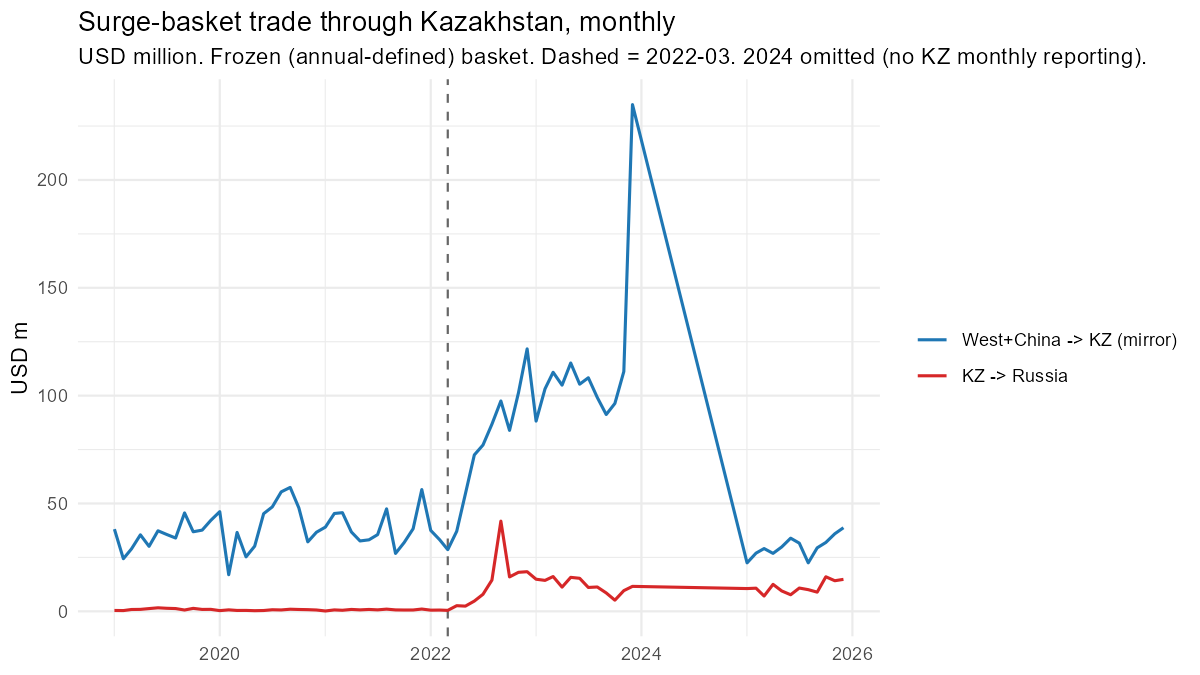
\includegraphics[width=.92\textwidth]{rq1_fig_monthly.png}
\caption{Surge-basket trade through Kazakhstan, monthly. USD million; blue = West + China
mirrored exports to Kazakhstan, red = Kazakhstan's exports to Russia. 2024 omitted (no
Kazakhstan monthly reporting to Comtrade). Dashed line: March 2022. Source: UN Comtrade.}
\label{fig:monthly}
\end{figure}

\begin{figure}[t]
\centering
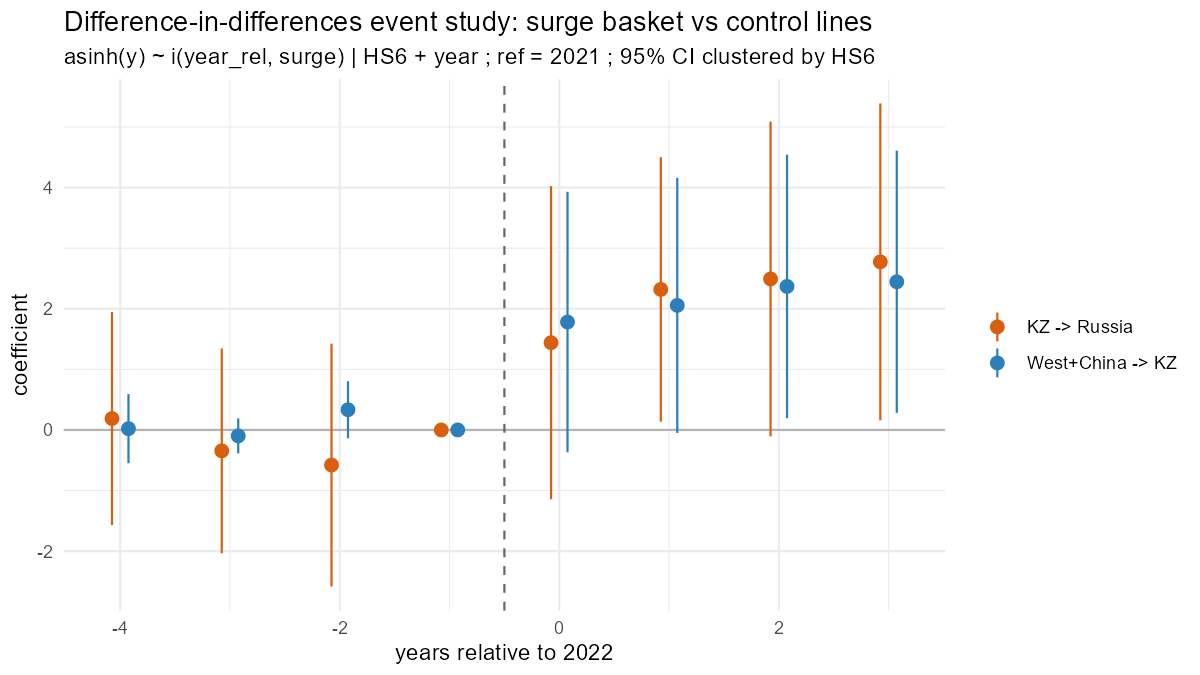
\includegraphics[width=.92\textwidth]{rq1_fig_eventstudy.png}
\caption{Difference-in-differences event study, surge basket vs.\ control lines:
$\text{asinh}(y_{it}) = \sum_{k\neq -1}\beta_k\,(\text{surge}_i \times \mathbf{1}[t - 2022 = k])
+ \mu_i + \lambda_t + \varepsilon_{it}$, HS6 and year fixed effects, 95\% confidence intervals
clustered by HS6, reference year 2021. Source: UN Comtrade.}
\label{fig:es}
\end{figure}

\subsection{Difference-in-differences}\label{sec:did}

\paragraph{Specification and identifying assumptions.} On the annual panel we estimate
$\text{asinh}(y_{it}) = \gamma\,(\text{treated}_i \times \text{post}_t) + \mu_i + \lambda_t +
\varepsilon_{it}$ with HS6 and year fixed effects and standard errors clustered by HS6 (75
lines, 8 years; reference year 2021). Zeros are common on the outbound leg before the shock
and rare after (23\% of surge-basket cells are zero in 2018--21 against 3\% in 2022--25), so
we report the asinh specification alongside a Poisson (PPML) estimate in levels, which handles
the zeros without a transformation and weights by size; the two tell the same story
(Table~\ref{tab:did}). Identification requires parallel paths absent the shock
(a joint test of the three pre-period interaction coefficients does not reject: $p = 0.42$
inbound, $p = 0.78$ outbound) and no anticipation (dropping 2022 entirely, or setting the
treatment year to 2023, leaves $\gamma$ essentially unchanged; see below). The civilian
control lines are not perfectly clean: their exports to Russia also break in 2022
(see ``The reform confound'' below), so $\gamma$ is if anything attenuated relative to the
economy-wide effect. The surge basket is \emph{selected on the post-period outcome}, which inflates $\gamma$
mechanically; the selection-rule-matched permutation test below, not the cross-sectional
regression, is what speaks to this and to the cross-sectional dependence a single common
treatment date induces. We also report wild-cluster-bootstrap $p$-values (few clusters,
within-HS6 serial correlation) and Holm-adjust across the four surge-basket outcomes. Both the
analytic and the bootstrap standard errors cluster within HS6 but treat lines as independent;
with a single common treatment date and a shock that hits related product lines together, that
is optimistic. The randomisation-inference $p$-values below do not rely on it (they resample
whole treatment histories) and are the inference we lean on.

\paragraph{Results.} Table~\ref{tab:did} reports $\gamma$ for the surge basket, the
externally defined priority list, and a placebo. On the surge basket, exports to Russia rise by
$\gamma = 2.44$ ($p = 0.013$; wild-bootstrap $p = 0.010$; Holm-adjusted $p = 0.039$; Poisson
in levels $3.5\times$, $p = 0.02$). The inbound flow (West + China) rises by
$\gamma = 2.10$ ($p = 0.05$, not significant after Holm adjustment); the Western component
alone by $1.73$ ($p = 0.08$); Kazakhstan's own reported imports by $1.88$ ($p = 0.004$, Holm
$p = 0.016$). The externally defined priority list, which is not selected on the Kazakh outcome, gives the
same pattern ($\gamma = 2.88$ outbound, $2.12$ inbound). The outbound effect survives two
further checks: adding size-decile$\times$year fixed effects (pre-2022 inbound size) leaves
$\gamma = 2.29$ ($p = 0.003$), and dropping 2022 raises it to $2.71$ ($p = 0.012$). The same
size$\times$year controls cut the West + China inbound coefficient to $1.28$ ($p = 0.05$),
consistent with the inbound leg being the weaker of the two throughout. Tightening the
selection threshold from a doubling to $2.5\times$ or $3\times$ raises the outbound
$\gamma$ to about $3.1$. Loosening it to $1.5\times$ (40 lines) lowers it to $1.6$
($p = 0.08$). A leave-one-HS2-out jackknife shows the effect is carried by HS~85: dropping it
(13 of the 29 lines) leaves $\gamma = 1.36$ ($p = 0.21$); the other six chapters, dropped one
at a time, give $\gamma = 2.51$ (drop HS~39), $2.48$ (HS~40), $2.67$ (HS~61), $2.28$
($p = 0.06$; HS~84), $3.16$ (HS~90) and $2.59$ (HS~96), all significant at 5\% except HS~84 at
6\%. The point estimate thus depends materially on the electrical-machinery lines, which is
where the reorientation is concentrated; the sign and the sub-5\% significance do not, except
when the largest chapter is removed.

Three qualifications keep us from resting identification on this cross-sectional
regression (the full battery is in Appendix~\ref{app:did}). First, the selection-rule-matched
permutation: when we impose the null by permuting
the year labels within each HS6 and re-applying the doubling rule, the rule selects on average
five lines (never as many as the 29 observed, so the \emph{existence} of the surge basket is
not a chance artefact, $p < 0.001$); a trend-preserving version that only shifts the break off
calendar-2022, keeping each line's autocorrelation and level trend, gives the same result
(null mean five lines, $p < 0.001$), so it is the 2022 alignment and not a pre-existing trend
that the selection picks up. But the observed $\gamma = 2.44$ sits squarely inside the
rule-matched null distribution of the coefficient itself (null mean $2.79$, s.d.\ $1.50$;
$p = 0.58$ for $|\gamma^{\text{perm}}| \ge |\gamma^{\text{obs}}|$), so the coefficient's
\emph{magnitude} is not separable from the selection and we do not read it as an identified
effect size. Second, the two
selection thresholds bind differently: 55 of the 75 candidate lines clear the outbound
doubling but only 41 clear the inbound one, so requiring both is a real screen on the import
side, not just on the outflow to Russia; this is a partial check against selecting the basket
purely on the outbound outcome that the difference-in-differences then uses. Third, the placebo row:
assigning fake treatment to the largest civilian lines gives $\gamma = -0.95$ ($p = 0.001$;
the large consumer-goods lines contracted after 2022 as the tenge depreciation would predict),
which shows the control pool is not homogeneous in trend. The surge coefficient's survival
of the size-decile$\times$year controls addresses this, and we do not read the placebo as
corroboration. Taken together, the cross-sectional difference-in-differences documents the
outbound reorientation but does not identify it on its own; the structural breaks
(Section~\ref{sec:shock}) and the neighbour comparison below carry that weight. The mirror-gap
outcome (partner-reported inflow minus Kazakh-reported imports) does not move
($\gamma = 0.54$, $p = 0.81$).

\begin{table}[t]
\centering
\caption{Difference-in-differences: $\gamma$ on $\text{treated}\times\text{post}$ in
$\text{asinh}(y_{it}) = \gamma(\text{treated}_i\times\text{post}_t) + \mu_i + \lambda_t +
\varepsilon_{it}$, HS6 and year fixed effects, cluster-robust standard errors (by HS6) in
parentheses. Surge-basket and priority-list rows have $N = 600$ (75 lines $\times$ 8 years);
the placebo row has $N = 200$ (the 25 civilian lines). The surge basket is selected on the
inbound (West + China) and outbound flows; the priority list (50 codes) is externally defined.}
\label{tab:did}
\footnotesize
\setlength{\tabcolsep}{5pt}
\begin{tabular}{@{}lcccc@{}}
\toprule
& Exports to & Inbound & Inbound & KZ-reported \\
Treated set & Russia & (W+China) & (Western) & imports \\
\midrule
\multicolumn{5}{@{}l}{\emph{Panel A. asinh DiD, $\gamma$ (cluster-robust s.e.\ by HS6)}} \\
Surge basket (29 HS6)                 & 2.44 (0.96)$^{*}$ & 2.10 (1.06) & 1.73 (0.98) & 1.88 (0.63)$^{**}$ \\
Priority list, external (50 HS6) & 2.88 (0.74)$^{***}$ & 2.12 (0.71)$^{**}$ & 1.93 (0.67)$^{**}$ & 2.94 (0.53)$^{***}$ \\
Placebo (largest civilian lines)      & --- & $-0.95$ (0.25)$^{**}$ & --- & --- \\
\midrule
\multicolumn{5}{@{}l}{\emph{Panel B. Poisson (PPML) DiD in levels, $e^{\beta}$ (multiplicative)}} \\
Surge basket (29 HS6)                 & $3.5\times^{*}$ & $2.4\times^{***}$ & --- & --- \\
\midrule
\multicolumn{5}{@{}l}{\emph{Panel C. selection-rule-matched randomisation inference (surge basket, exports to Russia)}} \\
\multicolumn{5}{@{}l}{\quad rule-matched null $\gamma$: mean $2.79$, s.d.\ $1.50$; $P(|\gamma^{\text{perm}}|\ge 2.44) = 0.58$} \\
\multicolumn{5}{@{}l}{\quad basket-existence null: $P(\text{rule selects}\ge 29\text{ lines}\mid H_0) = 0.000$} \\
\bottomrule
\end{tabular}

\vspace{2pt}
\footnotesize $^{*}$ $p<0.05$, $^{**}$ $p<0.01$, $^{***}$ $p<0.001$ (cluster-robust; before
multiple-testing adjustment). After Holm adjustment across the four surge-basket outcomes,
exports to Russia and KZ-reported imports remain significant at 5\%. Surge-basket and
priority-list rows in Panel A have $N = 600$ (75 lines $\times$ 8 years); the placebo row has
$N = 200$. Panel B: exact PPML coefficients $\beta = 1.26$ ($p = 0.02$) outbound and
$\beta = 0.85$ ($p < 10^{-4}$) inbound. Panel C: the coefficient's \emph{magnitude} is not
separable from the post-outcome selection, but the \emph{existence} of a 29-line basket is not
a chance artefact under either a free or a trend-preserving permutation.
\end{table}

\paragraph{The reform confound.} Three things separate the reorientation from the
outward-oriented policy agenda of 2022. First, the civilian control basket tells the story a
broad reform cannot: on the annual data its inbound flow shows no 2022 movement at all, and
while its exports to Russia do shift (a general Russia-trade effect), the shift is far
smaller than the surge basket's on the same test, and the monthly surge-basket outbound break
is much sharper still; the cross-sectional placebo runs the wrong way. Second, the outbound
break is dated 2022m5, before the June referendum and the November election. Third, and most
directly: Armenia's surge-basket exports to Russia rose from \$7--15m per year to \$71m in
2022 and \$93m in 2023, and the Kyrgyz Republic's from \$1--7m to \$12m and \$30m, on the same
timing, neither country having a ``New Kazakhstan'' reform. The direction is also the right one: the
goods come in from Western reporters and move onward to Russia, not the reverse.

\section{What Kazakhstan retains}\label{sec:capture}

\subsection{The retained trade margin}

We measure what Kazakhstan retains on the \emph{incremental} flow (exports to Russia above
the pre-2022 baseline, about \$479m cumulatively over 2022--2025), since that is the part the
reorientation drove. The \$479m increment is measured against a flat counterfactual at the
2018--21 mean (\$11m/yr); because the pre-2022 outbound series is itself declining
(\$17m$\to$\$8m), that is the conservative choice: extrapolating the pre-trend would put the
counterfactual near zero by 2024 and raise the increment to about \$521m, widening every
downstream figure by roughly a tenth. Set against the incremental \emph{Western} inbound of
about \$887m, the flow-through is roughly one half; set against the incremental West + China
inbound of about \$3.2bn, it is one sixth.\footnote{Three flow-through ratios appear in this
section, on different samples and bases: the \emph{incremental} ratio against the Western
inbound ($\approx 0.54$) and against West + China ($\approx 0.15$, ``one sixth'') used here,
both on aggregate 2022--25 minus baseline; and the \emph{matched-cell} aggregate ratio
($\approx 0.11$, sum of re-export value over sum of inbound value across the 112 matched
HS6$\times$period cells) used in the weight-ratio discussion below.} The inbound leg is the more weakly identified of
the two (its DiD coefficient loses significance under size$\times$year controls and after
multiple-testing adjustment, Section~\ref{sec:did}), so the flow-through ratio should be read
as indicative, not precise. The remaining \$887m${}-{}$\$479m${}={}$\$408m of
the Western increment decomposes into only about \$41m of onward exports to destinations other
than Russia (Kazakhstan's surge-basket exports to the rest of the world barely move) and about
\$367m of domestic absorption, inventory and the c.i.f./mirror measurement gap, so the
flow-through gap is not hidden re-export through third countries. The Western basis is the
relevant one for the reorientation, and we use it here.

The unit-value evidence is consistent with a corridor and does not identify a retained margin
on its own. On a c.i.f./f.o.b.\ basis (Kazakhstan's f.o.b.\ re-export price against the
c.i.f.\ price it records paying on import, which includes freight into a landlocked
economy), the median ratio across matched HS6$\times$period cells is \textbf{0.73} (annual,
$n = 112$; $0.70$ monthly). On a like-for-like f.o.b.\ basis, against the exporter-reported
price at the partner's border, the median is \textbf{1.6} (annual; $1.5$ monthly), the
difference being roughly the inbound freight. Neither ratio is distinctive (the civilian
control basket gives $0.59$ and $0.94$ on the two bases), and the pass-through regression is
weak on both (a slope of $0.06$--$0.48$, significant only in the annual f.o.b.\
specification).

Two features cut against domestic transformation, though neither is decisive. The first is the
weight ratio (re-exported tonnage over imported tonnage in the matched cell), which is
$0.08$ at the median and $0.11$ in aggregate, close to the matched-cell value flow-through
(median $0.15$, aggregate $0.11$). The aggregate weight ratio and the aggregate value
flow-through are the same statistic on different units and coincide here at $0.11$, so a
sub-one weight ratio is largely a flow-through fact, given that only part of the imported
tonnage is re-exported to Russia at all, and is not evidence on weight gain per transiting
unit. Eleven per
cent of cells do carry a weight ratio above $1.05$, on a wide interquartile range ($0.02$ to
$0.49$); under the flow-through reading that upper tail is timing and inventory rather than
processing. Restricting to the six near-pure-transit HS6$\times$period cells where value
flow-through is near one, the weight ratio is $0.74$ at the median ($0.26$ and $0.94$ at the
quartiles, on $n = 6$), showing no sign of local input added on the goods that do transit,
though on a thin slice of the basket. The
Comtrade extract as pulled carries value and net weight but not physical quantity, so a
cleaner per-unit transformation test is not available here.

The second feature is the dispersion in the f.o.b.\ wedge, which is not a processing signal.
The wedge is uneven across tiers,\footnote{The priority list is
published with the goods grouped into tiers (Tier~1--2 the most sensitive, Tiers~3--4
progressively less so); we carry the published tier labels unchanged and use them only to
describe where in the list the high wedges fall. Tier~1 = HS 8542 (integrated circuits);
Tier~2 adds transceivers, capacitors, connectors; Tiers~3--4 are broader machinery,
instruments and components.} with tier medians near four in Tiers~2 and~4A but around one in
Tiers 3B and 4B and only $0.47$ in Tier~1; the high multiples sit on about half the matched
gross flow (Figure~\ref{fig:wedge}). An uneven wedge concentrated in a subset of lines is the
pattern of a scarcity markup on goods that became harder to source directly, not the even,
across-the-board wedge a processing margin would produce. It is the pattern
\citet{feenstrahanson2004entrepot} document for Hong Kong's entrep\^ot trade in Chinese goods,
where the re-export markup is largest where the intermediary adds matching and
scarcity value rather than physical transformation; the wedge here is if anything smaller and
noisier. The value-weighted aggregate wedge is below one, dominated by a handful of
high-inbound-value cells and by outbound under-invoicing \citep{fisman2004missing}. The wedge
does not pin the retained margin, which we take from the national accounts next.

\begin{figure}[t]
\centering
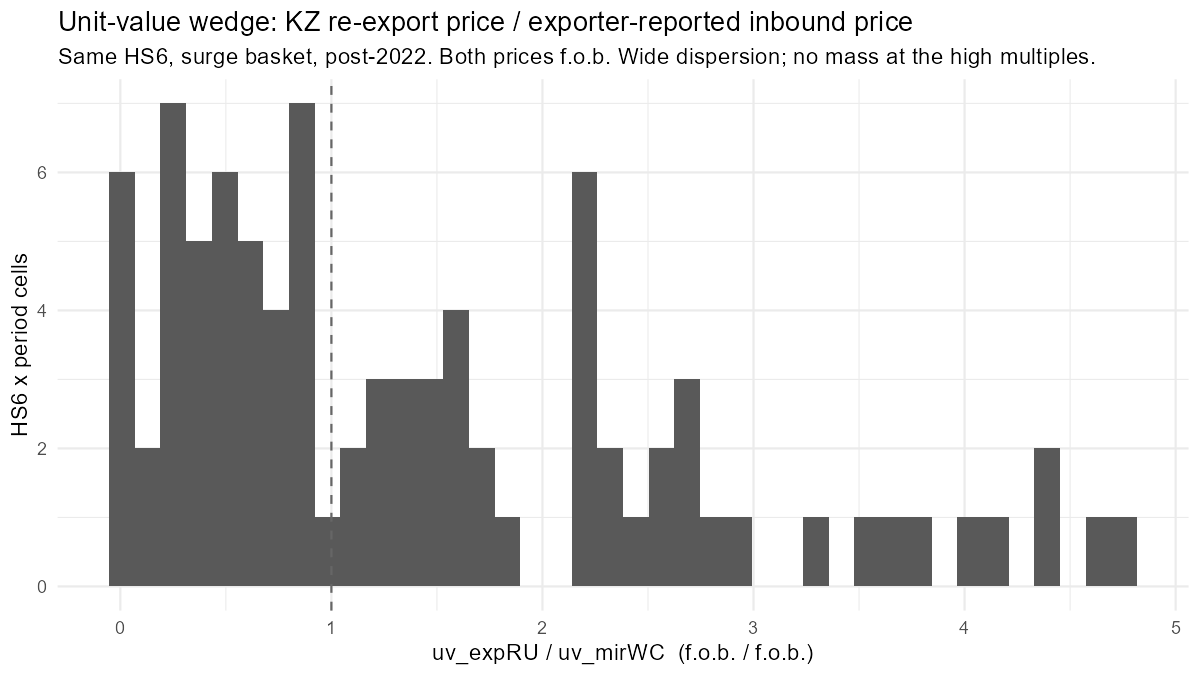
\includegraphics[width=.72\textwidth]{rq2a_fig_wedge_hist.png}
\caption{Unit-value wedge: Kazakhstan re-export price over the exporter-reported inbound price
(f.o.b.\ basis), same HS6, surge basket, post-2022. Wide dispersion, with the high multiples
falling in a subset of lines (tier medians near four in Tiers~2 and~4A, around one elsewhere):
the pattern a scarcity markup produces, not the even, across-the-board wedge a processing
margin would.}
\label{fig:wedge}
\end{figure}

\subsection{Input--output propagation}

Let $m$ be the trade-and-freight margin Kazakhstan retains on a transiting good as a share of
its value, $\bar v^{TT}$ the mean domestic value-added multiplier for its trade, transport and
warehousing sectors, and $\bar v^{M}$ that for manufacturing. Domestic value added per dollar
of gross rerouted flow is $m\,\bar v^{TT}$; per dollar of domestic manufacturing output it is
$\bar v^{M}$ \citep{koopman2014tracing,johnson2012accounting}. From the OECD ICIO Kazakhstan
block, $\bar v^{TT} = 0.79$ and $\bar v^{M} = 0.76$, close enough that the propagation step
does little work: the result is essentially $m$ against the full domestic value $\bar v^{M}$.

We take $m$ to be what a trading intermediary retains when it buys a good wholesale and
re-sells it without a retail leg or a physical transformation: the c.i.f./f.o.b.\ freight and
insurance wedge plus a wholesale (not retail) trade margin. The Kazakhstan Bureau of National
Statistics resources table \citep{qazstat2023io} bounds it: the \emph{transport} margin on
machinery and electronics is about 1\% of basic-price value, and the \emph{full}
trade-and-transport margin (which also carries the retail leg the corridor never performs) is
about 49\%. A wholesale-plus-freight margin sits in the lower part of that range. The
freight-and-insurance wedge between an f.o.b.\ and a c.i.f.\ price is conventionally a few per
cent (the c.i.f./f.o.b.\ factor applied in trade statistics is about 1.06); recorded
c.i.f./f.o.b.\ margins for former-Soviet economies are too noisy to use directly, and for
several the recorded f.o.b.\ figure exceeds the c.i.f.\ one \citep{arvis2010landlocked}, so we
do not lean on them. Adding a wholesale distributive margin of a few points to a single-digit
freight wedge gives the lower half of the Bureau of National Statistics bracket. We use \textbf{6--14\%} and treat it as a
calibration, not an estimate:
because
$\bar v^{TT} \approx \bar v^{M}$ the input--output step does no work, so the headline is a
direct function of $m$ and we carry it as a band. (We do not use the matched-cell unit-value
wedge to pin $m$: censoring negative-margin cells inflates the gross margin to about 34\%,
while the value-weighted aggregate is negative, and both are artefacts of the c.i.f./f.o.b.\
basis mismatch and of outbound under-invoicing rather than measures of domestic value
retained.)
Domestic value added per dollar rerouted is then $m\,\bar v^{TT} \approx$ \textbf{5--11\%},
midpoint about \textbf{8\%}, against \textbf{76\%} per dollar of domestic manufacturing
output, so a rerouted dollar creates on the order of a tenth as much domestic value as a
produced one. Of the \$479m in incremental exports to Russia after 2022, Kazakhstan retains
roughly \textbf{\$23--53m} as domestic value added.

Because the propagation step is close to the identity, the headline is a one-for-one function
of $m$, and the reader can substitute a different margin directly (Appendix~\ref{app:io}
gives the full sweep, the input--output cross-check and the matched-cell wedge detail).
Sweeping $m$ across the full
Bureau of National Statistics bracket: at the transport-only end ($m \approx 1\%$) a rerouted
dollar captures about one-hundredth of a produced one; across our $6$--$14\%$ band, one-sixteenth
to one-seventh; the ``corridor, not factory'' reading (a rerouted dollar worth on the order of
a tenth of a produced one) holds for any $m$ up to about $12\%$. It weakens to ``about a fifth''
only at $m \approx 19\%$, to ``about a third'' at $m \approx 32\%$, and reaches about a half
only at $m \approx 49\%$, the full trade-and-transport margin that includes the retail leg the
corridor never performs. The censored matched-cell gross margin ($34\%$), even taken at face value, still
leaves a rerouted dollar at about a third of a produced one. The qualitative conclusion is thus
robust to any margin a wholesale-plus-freight reading can support; it fails only if the corridor
in fact captures a near-complete retail-inclusive markup. The one piece of evidence that bears
directly on a markup that large is the value-weighted aggregate unit-value wedge, which is
itself below one; we read that as suggestive only, because it is depressed by
outbound under-invoicing and the c.i.f./f.o.b.\ basis mismatch.

The multipliers matter little by comparison. Even at $\bar v^{M} = 0.40$ the ratio is about one
to five; recomputing $\bar v^{TT}$ and $\bar v^{M}$ from the Bureau of National Statistics
symmetric input--output table (68 products, 2023) rather than the OECD ICIO gives
$\bar v^{TT} = 0.89$ and $\bar v^{M} = 0.74$, moving the rerouted-vs-produced ratio from about
one-in-ten to one-in-eight, still an order of magnitude. Under-invoicing moves it only so far:
for domestic value added to reach one-fifth \emph{of the gross rerouted flow} (a looser
benchmark than one-fifth of a produced dollar, which $m \approx 19\%$ already breaches), the
trade margin would have to be about $25\%$, which, holding the recorded import cost fixed,
requires exports to Russia to be under-recorded by $13$--$21\%$. Under-recording on that scale is within the range found for
transit trade \citep{fisman2004missing} and cannot be excluded; but even at that bound
Kazakhstan retains at most about a quarter of what a producing economy captures.

\subsection{Fiscal and macro}

The reorientation-attributable flow (incremental exports to Russia over the pre-2022
baseline) is about \$479m cumulatively over 2022--2025 (\$107--134m per year). Customs duty on
it, at an EAEU common external tariff of 4--8\% on the share formally cleared in Kazakhstan, is
on the order of \textbf{\$22m over four years} (about \$5m per year); net import VAT is close
to zero because the onward supply to Russia is intra-union and zero-rated. Kazakhstan's annual
customs revenue is of the order of \$4--5bn, so the reorientation adds well under 1\%. At the
macro level the flow is 0.2--0.3\% of GDP; the 2022 current-account surplus, the reserve
accumulation of 2023--2025 and the rise in services value added are an order of magnitude too
large to be driven by it.

\section{The (non-)investment response}\label{sec:investment}

If the demand shock were seeding domestic value added, we would expect a rise in investment
in the sectors the flow passes through. We find none, though with only four post-2022 years
the deal-count test can rule out only a large response, not a modest one.

Deal-making in manufacturing of tradeable goods, transport and logistics, and wholesale
distribution runs at \textbf{7.6 per year} in 2015--2021 and \textbf{7.2 per year} in
2022--2025 (a Poisson rate ratio of 0.96, 95\% CI 0.59--1.53). The two thinnest years are
2015, with a single recorded deal as the databases ramp up their Kazakhstan coverage, and
2022, the unrest year (Figure~\ref{fig:mismatch}). Excluding the thin 2015 first year the
pre-2022 rate is 8.7 per year, so the post period is a slight decline on either basis. Dropping the 2022 trough,
2023--2025 runs at 8.7 per year (rate ratio 1.14, 95\% CI 0.69--1.86). The test has 80\% power
only against an increase of roughly 80\% or more, so it excludes a surge in deal-making but
not a modest step-up. The composition of that activity says more than the count. Reported deal
\emph{value} in these sectors rises, but it is concentrated in ownership transfers of existing
or distressed assets, not new productive capacity: the ArcelorMittal Temirtau to Qarmet
nationalisation (2023), Eurocopter Kazakhstan and the Lokomotiv rolling-stock plant
(re-nationalisations, 2024), and a \$0.8bn 2025 consolidation of rail-freight and forwarding
assets. Greenfield and new-capacity transactions average under two per year and never exceed
four, with no post-2022 increase. And across the whole
2015--2025 window the data contain \textbf{no} transaction in the specific product lines that
dominate the reorientation, though we do not lean on this, because the pre-2022 base rate in
those narrow lines is also near zero, so the post-period zero carries little information on its
own. We would have coded as a positive investment
response any greenfield or capacity-expansion deal, in any of the three databases, tagged
to a surge-basket HS6 \emph{or} to its parent electrical-machinery, components or
instrument-manufacturing class. On that rule the count is zero before and after, and the
informative statistic is the sector-level rate test above, which rules out a step-up of about
a doubling or more.

\begin{figure}[t]
\centering
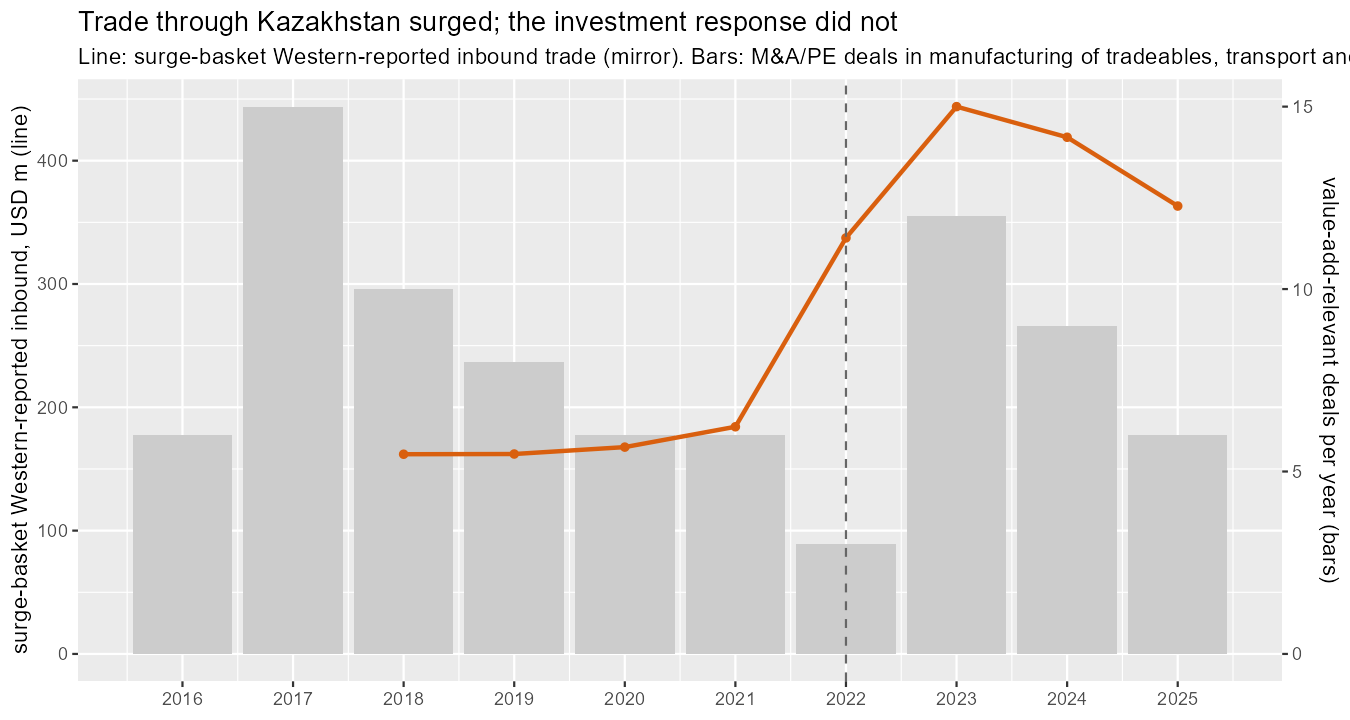
\includegraphics[width=\textwidth]{valueadd_fig_mismatch.png}
\caption{Trade through Kazakhstan surged; the investment response did not. Line:
surge-basket \emph{Western-reported} inbound trade (partner-reported mirror), USD million
(left axis; the West + China total is several times larger but was already growing before
2022). Bars: annual count of M\&A/PE deals in manufacturing of tradeable goods, transport and
logistics, and wholesale distribution (right axis). Dashed line: 2022. Bars shown from 2016;
2015 has a single recorded deal and is omitted (Section~\ref{sec:investment}). Source:
UN Comtrade; Capital~IQ/PitchBook/Preqin.}
\label{fig:mismatch}
\end{figure}

The result holds across the three databases. Table~\ref{tab:dealsource} reports deal counts
for the same Kazakhstan universe from each source; coverage differs in level (the
transaction-oriented Capital~IQ extract records more mid-market M\&A, the venture-heavy
PitchBook more small early-stage rounds, Preqin fewer of either), but none shows more than a
flat rate in manufacturing or logistics deal-making (5.1 to 5.2, 2.0 to 1.5, and 0.4 to 0.5
per year). In the Capital~IQ extract, which best
captures the mid-market industrial deals that a genuine capacity response would generate, the
count of manufacturing, transport and distribution deals is essentially unchanged before and
after 2022 (5.1 versus 5.2 per year).

\begin{table}[t]
\centering
\caption{Deal counts for the Kazakhstan universe, by source and period. Rates are per year
over a 7-year pre-window (2015--21) and a 4-year post-window (2022--25). The consolidated
non-duplicate universe is $N = 493$ transactions; the manufacturing, transport and
distribution subset is $N = 82$ (53 pre, 29 post).}
\label{tab:dealsource}
\footnotesize
\begin{tabular}{lrrr}
\toprule
Deals per year (unless noted) & Cap.~IQ & PitchBk & Preqin \\
\midrule
All deals, 2015--21              & 24.0 & 14.6 & 3.7 \\
All deals, 2022--25              & 23.2 & 24.2 & 1.8 \\
Mfg + transport + distrib., 2015--21 & 5.1 & 2.0 & 0.4 \\
Mfg + transport + distrib., 2022--25 & 5.2 & 1.5 & 0.5 \\
Surge-basket lines, 2015--25 (total) & 0$^{a}$ & 0 & 0 \\
\bottomrule
\end{tabular}

\vspace{2pt}
\footnotesize $^{a}$ Two Capital~IQ records carry an ``electronic'' industry tag (a
steel-wire-rope manufacturer and a finance holding company) and are misclassifications; there
are no transactions in the reorientation's product lines.
\end{table}

Kazakhstan is adding vehicle assembly (Chinese marques, KIA, \v{S}koda) and some appliance
capacity, but this predates and is largely independent of the reorientation, is kit assembly
with low domestic value added, and serves the domestic and Eurasian consumer market rather
than the re-export flow to Russia. The state investment corporation's disclosed
post-2022 pipeline is domestic food, energy and infrastructure, not corridor processing
\citep{qicaifcifc2026pe}. The one
investment signal that is reorientation-linked, a 2025 consolidation of cross-border
rail-freight and forwarding assets, deepens Kazakhstan's role as a forwarding operation, not
a producing one.

\section{Which gate binds?}\label{sec:why}

Equation~\eqref{eq:gates} attributes the null to at least one factor near zero.
The market-access gate is open: under the Eurasian Economic Union the good moves to
Russia with no transformation and no border, so $V_T > 0$, and because a domestic plant's
transformation margin sits below the thin re-export markup ($\mu_P \lesssim \mu_T$, on the
sector's near-zero domestic base and its $0.69$ value-added multiplier, Section~\ref{sec:framework}),
building is dominated in \eqref{eq:build} before the option value is added. The re-export flow
is not distinguishable in price or weight from ordinary Kazakh trade
(Section~\ref{sec:capture}). In a multiplicative decomposition an open market-access gate is
close to sufficient for $R \approx 0$ on its own, which limits what the case can say about
the other two gates: we observe a single configuration, with no gate clearly favourable and
the three not separately identified. What we can add is a state-fund pipeline that rules the
institutional gate out as the binding constraint for this null (the least
capital-constrained investor in the economy did not build), and a
durable-versus-uncertain shock comparison that is suggestive of an adverse
irreversibility gate but confounded. Neither identifies a gate cleanly, and we set out the
limits of each below.

Kazakhstan's state
investment corporation (QIC\slash Baiterek) faces neither an external-finance nor an exit
constraint, so the institutional gate does not bind for it the way it binds for an outside
investor. Its deployment in fact \emph{rose} sharply after 2022: about \$2.2bn cumulative
over 2015--2025, some \$1.5bn of it in 2025, of which \$1.0bn was a single steel-producer bond
\citep{qicaifcifc2026pe}. But the projects the report identifies are a power plant, a poultry
producer, steel and energy bonds, a pipe-systems maker, a bioethanol plant, a school and an
office block: domestic food, energy and infrastructure, none in a surge-basket line
and none in corridor logistics built for the flow; the report's note that manufacturing became
prominent in the deal record from 2023 refers to these domestic-market projects. This is
illustrative rather than a controlled test (the report gives no pre-2022 baseline and no
sector-level denominator), but the least capital-constrained investor in the economy did not
build for the reorientation either.

Over the same window, and inside the same institutions, Kazakhstan's \emph{durable}
passenger-vehicle demand shock (Western marques withdrawing from
Russia, a domestic consumption boom, and Eurasian market access) was met with real capacity:
a combined Changan\slash Haval\slash Chery assembly facility of about 90{,}000 units, a KIA
plant (about \$200m), local assembly of several \v{S}koda models, and a car-multimedia plant
in Almaty (2024). The re-export shock was met with no plant at all. The comparison is
illustrative, not a controlled test. In the deal
databases auto-sector transactions actually \emph{fell} after 2022 (six in 2015--2021, three
in 2022--2025); the capacity evidence comes from plant announcements and public reporting,
and no symmetric announcement search was run for the component sector, so a searched sample is
being set against an unsearched one. Much of the auto capacity also predates the reorientation
(Section~\ref{sec:investment}). And the two shocks differ along several axes at once:
persistence and certainty, sunk-cost intensity, whether market access requires domestic
content (EAEU local-content rules bind for vehicles but not for the re-export, so the
comparison also moves the market-access gate), and the destination market. The pattern is
consistent with a durable, transformation-requiring shock drawing capacity where a re-export
shock does not; it is not an experiment on any single gate.

A 2022 entrant faced an uncertain shock, not an observed transitory one. The flow to Russia
peaked in September 2022 and fell by more than a third over the second half of 2023, from
about \$15m per month in 2023-H1 to about \$9m in 2023-H2, as trade-monitoring measures
tightened (the EU's eleventh sanctions package, Council Regulation (EU) 2023/1214 of 23 June
2023, introduced a transit-monitoring provision). But that within-year decline is a correction
from the September-2022 spike to a plateau, and not a decay path: on the \emph{annual} series
exports to Russia in these lines run \$128m, \$145m, \$119m and \$133m across 2022--2025,
roughly ten times the pre-2022 baseline, with no downward trend and 2025 above 2024
(Table~\ref{tab:magnitudes}; with monthly reporting suspended after February 2024 and resumed
only in 2025, the sub-annual path across the 2024 transition is not observed). \emph{Ex post} the flow
persisted; what a 2022 entrant faced was high \emph{uncertainty} about its duration. The flow
is policy-contingent (successive sanctions packages, monitoring provisions, compliance
exposure) and its duration was unknowable. In the framework's terms this is a high-$\sigma$
configuration, which raises $\Omega$ and delivers the same null as a low-$\rho$ one; we do not
claim the realised persistence was low.

The state fund's pipeline
rules the institutional gate out for the \emph{shock-specific} null, but there is one place in
the case where a single gate varies while the others hold, and it points to institutions: the
durable adjacent opportunities of Section~\ref{sec:where}, for which the irreversibility gate
is plausibly open (warehousing and transport support, with a domestic value-added multiplier
of 0.82; machinery and fabricated-metal import substitution), are also financed only slowly
and only by directed state capital. An open irreversibility gate with no private investment
response is evidence that the institutional gate binds \emph{there}. The domestic
private-equity market has no functioning exit, with the founder buy-back the leading route
\citep{qicaifcifc2026pe}; capital is dominated by state and
development-finance money, and the 2022--2025 pipeline is crowded by nationalisations. This is
the institutional-voids configuration of \citet{khannapalepu2000} and \citet{rajanzingales1998}, and
it is the subject of related work.

\section{Moderators and external validity}\label{sec:moderators}

The decomposition organises seven moderators, listed in
Table~\ref{tab:moderators} with the value each takes for Kazakhstan. Its empirical content is
in the three necessary conditions, not in the functional form of \eqref{eq:gates}: $R$ is
positive only when the market-access gate is closed to a pure re-export and the irreversibility
gate is open, and large only
when the institutional gate is open as well. A country adverse on the first two should show a
null irrespective of its institutions, and a country favourable on all three should show a
supply response even with a shallow capital market.

\begin{table}[t]
\centering
\caption{Moderators of the investment response, and Kazakhstan's values}
\label{tab:moderators}
\small
\begin{tabular}{@{}p{5.4cm}p{2.3cm}p{3.1cm}c@{}}
\toprule
Moderator & Gate & Kazakhstan, 2022 & $R\!\uparrow$ when \\
\midrule
Shock persistence $\rho$ (structural reallocation vs.\ event-driven) & irreversibility & flow persisted \emph{ex post}; \emph{ex ante} uncertain & high \\
Uncertainty $\sigma$ / policy risk & irreversibility & high (policy-contingent) & low \\
Sunk-cost intensity $I$ of the relevant technology & irreversibility & high (component mfg) & low \\
Domestic transformation required to reach the market (rules of origin, local content, a border) & market access & none (customs union) & required \\
Financial depth / exit availability & institutions & shallow, no exit & deep \\
Private vs.\ state / directed capital mix & institutions & state-dominated & private-led \\
Existing productive base / absorptive capacity & institutions & near-zero (electronics output $\approx$ \$230m) & a base exists \\
\bottomrule
\end{tabular}
\end{table}

Within the reorientation group, Armenia and the Kyrgyz Republic received the same
shock, with surge-basket exports to Russia rising several-fold and breaking in 2022 on the
same timing, and they share Kazakhstan's value on every moderator: the shock is event-driven,
its persistence uncertain \emph{ex ante}, policy risk is high, and the customs union removes
the need to transform. Two features are informative. Both neighbours' flows had already
receded by 2024--2025 (Armenia's surge-basket exports to Russia: \$71m, \$93m, \$42m, \$13m
over 2022--2025; the Kyrgyz Republic's \$12m, \$30m, \$12m, \$12m), whereas Kazakhstan's
persist (\$128m, \$145m, \$119m, \$133m). The neighbour reversion shows the flow could recede,
and the Kazakhstan asymmetry means the ``same shock'' claim holds for the 2022--2023 surge
but not for its persistence. And we do not have deal-level data for Armenia
or the Kyrgyz Republic (our commercial extracts are Kazakhstan-only), so we cannot test the
investment null for them directly; what we can say is that neither has a domestic
component-manufacturing sector to expand.

Outside the customs union, the named population of post-2022 intermediaries is
\{Kazakhstan, Armenia, the Kyrgyz Republic, Belarus\} inside the Eurasian Economic Union and
\{Georgia, T\"urkiye\} outside it. The distinction matters for the framework: a non-member
routes goods to Russia across a customs border, so its market-access gate is not fully open,
and the framework predicts it is the more likely of the two groups to see a domestic
processing or assembly response. On the trade side the shock is visible in the non-members
too: T\"urkiye's surge-basket exports to Russia roughly double at the 2022 break (from about
\$58m in 2021 to \$119m in 2022 and \$207m in 2023; sup-$F$ of $11.9$, $p = 0.007$), while
Georgia barely participates in this particular flow (under \$2m a year throughout, no clean
break); Appendix~\ref{app:breaks} gives the full series and break tests, alongside Armenia and
the Kyrgyz Republic. We cannot run the investment test for either: our deal data are Kazakhstan-only, and
T\"urkiye's large pre-existing manufacturing base would in any case make a marginal-capacity
response hard to detect in aggregates. The external-validity claim we can support is therefore
narrow: the \emph{demand shock} generalises across the intermediary population, while the
\emph{investment null} is established only for Kazakhstan, where the market-access gate is
fully open and a domestic component sector barely exists.

As motivating contrast cases, economies that drew capacity investment from a post-2020
tradeable demand shock did so with a favourable configuration on the first two gates, not
necessarily the third. Vietnam and Mexico received China-plus-one and nearshoring
reallocations widely read as \emph{structural} \citep[e.g.][]{juhaszlanerodrik2024}, and in
autos the tightening of rules of origin under the United States--Mexico--Canada Agreement made
domestic content a condition of market access (a closed market-access gate that forces
$V_T \to 0$). Both invested in capacity despite financial markets that are not uniformly deep. This is the
pattern the framework predicts: persistence and a transformation requirement do the work, and
financial development scales the response.

We cannot, however, separate the irreversibility and institutional
gates across countries. Doing so would regress sector-level greenfield investment on shock
persistence and financial depth in a panel of intermediaries and contrast cases. In the sample available
to us the two are collinear: Kazakhstan, Armenia, the Kyrgyz Republic and the other Caucasus
and Central Asian intermediaries are all financially shallow (private credit plus market
capitalisation of 24--66\% of GDP, all below the comparator median), and T\"urkiye is
financially deeper but has too large a pre-existing manufacturing base for a marginal-capacity
response to register. Country-level macro aggregates are too noisy to isolate a
response of this size, and in places run the other way:
Armenia's gross fixed capital formation rose about three points of GDP after 2022.
The argument leans on the within-country comparisons of Section~\ref{sec:why}; a
cross-country panel using greenfield-project data by sector is the natural extension.

\section{Where investment would raise value capture}\label{sec:where}

The reorientation is nonetheless informative for investment policy, because the trade data
reveal which products have proven demand and proven routes through Kazakhstan. Table~\ref{tab:priority}
sets three quantities side by side for the candidate sectors, namely the domestic value-added
multiplier, the import-substitution gap (imports relative to domestic output), and the
post-2022 growth in import demand, after removing the surge-basket lines from the
electronics-adjacent chapters; we read them jointly rather than collapsing them into a single
index (Figure~\ref{fig:priority}).

Two groups stand out. The \textbf{logistics platform} (warehousing and transport support, and
wholesale-trade infrastructure) has among the highest domestic value-added multipliers in the
economy (0.82) and is the corridor's binding constraint, given the high and unpredictable
overland logistics costs a landlocked transit economy faces \citep{arvis2010landlocked};
investment here creates
domestic value and holds it whether or not the Russia flow persists. \textbf{Import substitution} in
electrical equipment, machinery, fabricated metal products and chemicals is the second:
Kazakhstan imports six to eight times what it produces in electrical equipment and machinery
and roughly twice its output in the other two; the domestic value-added multiplier is around
0.80, and a nascent deal base exists. By contrast, localising
the surge-basket products is the worst option: computer, electronic and optical manufacturing
has among the lowest value-added multipliers in the economy (0.69, tied with motor-vehicle kit
assembly) and a near-zero domestic base.

\begin{table}[t]
\centering
\caption{Sector characteristics for value-adding investment, Kazakhstan. VA mult.\ =
domestic value-added multiplier $(v_d' L_d)_j$ from the OECD ICIO block; Output = gross output,
\$m; Imp./output = 2023 imports over domestic output; Imp.\ growth = ratio of 2023 to 2019
import value. Dashes: not applicable (platform sectors are not import-competing) or not
computed. Surge-basket HS6 are netted out of the electronics and machinery chapters. The
substitution rows are the four top-ranked candidates on a combined score (value-added
multiplier, import-substitution gap, import growth, deal base) out of $N = 13$ ranked
tradeable sectors; two platform and two ``avoid'' rows are shown alongside, so 8 of the 13
appear here and the full ranking is in the replication output.}
\label{tab:priority}
\small
\begin{tabular}{@{}p{1.5cm}p{5.4cm}rrrr@{}}
\toprule
& Sector & VA & Output & Imp./ & Imp. \\
& & mult. & \$m & output & growth \\
\midrule
\multirow{2}{1.5cm}{Platform}
 & Warehousing \& transport support & 0.82 & 6{,}800 & --- & --- \\
 & Wholesale \& retail trade infrastr. & 0.82 & 81{,}000 & --- & --- \\[2pt]
\multirow{4}{1.5cm}{Substi\-tution}
 & Electrical equipment & 0.81 & 1{,}150 & 5.6 & 1.43 \\
 & Machinery \& equipment n.e.c. & 0.80 & 1{,}160 & 7.9 & 1.27 \\
 & Fabricated metal products & 0.81 & 1{,}850 & 1.8 & 1.22 \\
 & Chemicals & 0.79 & 3{,}480 & 1.7 & 1.52 \\[2pt]
\multirow{2}{1.5cm}{Avoid}
 & Computer, electronic \& optical (surge basket) & 0.69 & 230 & --- & --- \\
 & Motor vehicles \& parts (kit assembly) & 0.69 & 1{,}530 & 6.1 & 2.55 \\
\bottomrule
\end{tabular}
\end{table}

\begin{figure}[t]
\centering
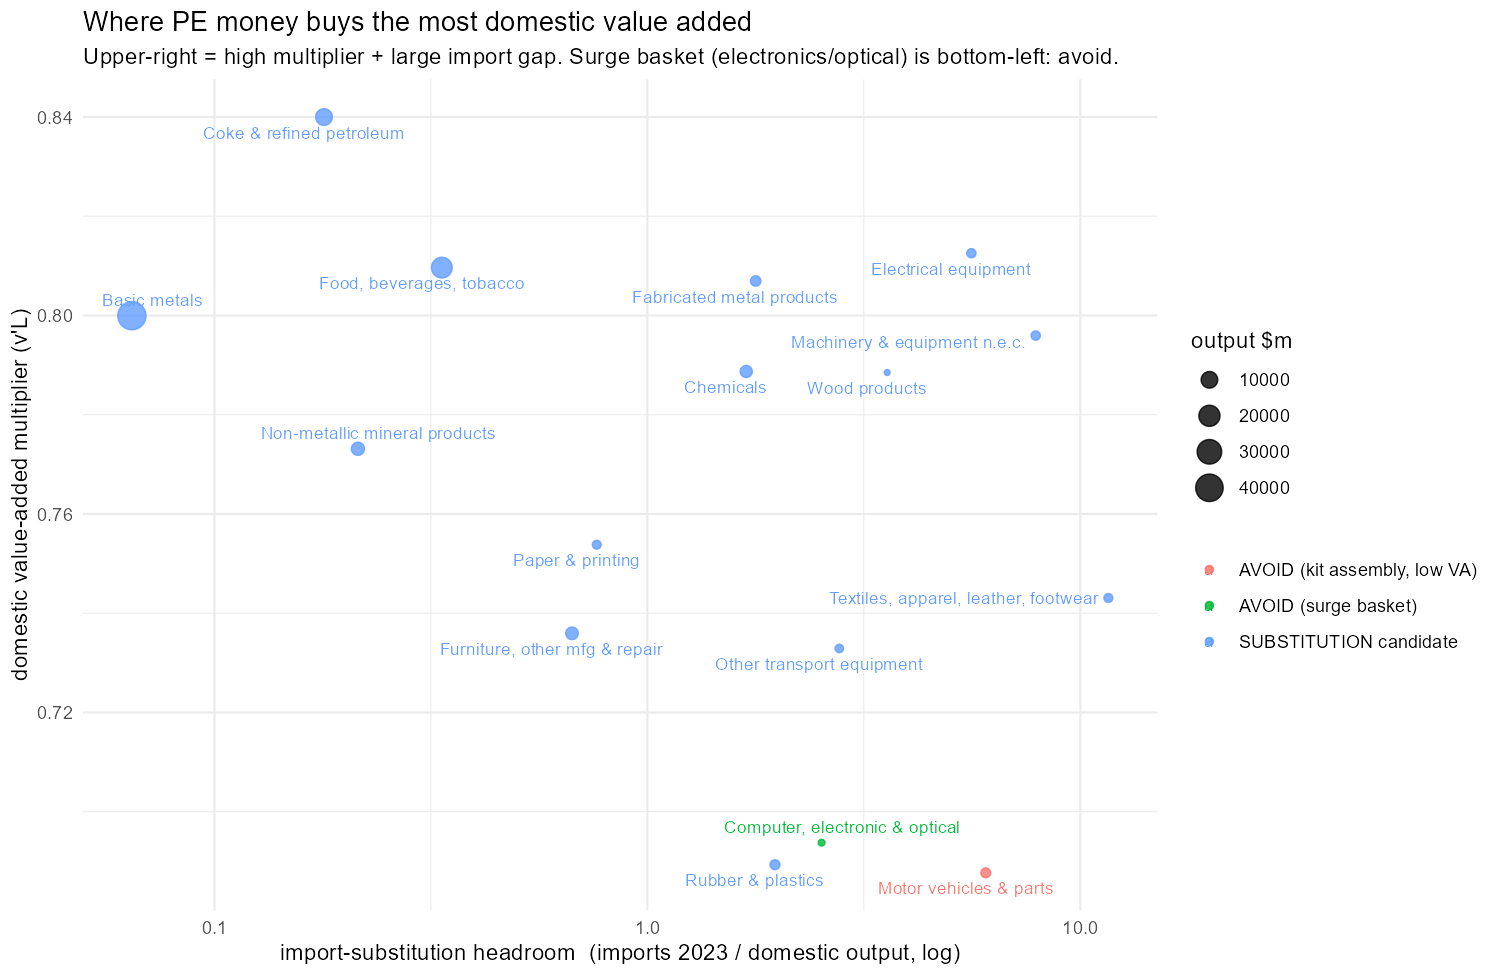
\includegraphics[width=\textwidth]{sector_priority_fig.png}
\caption{Where investment buys the most domestic value added: domestic value-added multiplier
against import-substitution headroom (imports 2023 / domestic output, log scale), bubble size
= domestic output. The surge-basket products (computer/electronic/optical) sit at the bottom.}
\label{fig:priority}
\end{figure}

These opportunities are investable at scale only if the state investment corporation shifts
from lead direct investor to co-investor behind private leads, with larger syndicated tickets
and a credible exit (trade sale or listing) rather than the buy-back that currently
dominates. That is a question about capital-market institutions, taken up in related work.

\section{Policy implications}\label{sec:policy}

The framework of Section~\ref{sec:framework} is also a menu of levers. A demand shock of this
kind industrialises a transit economy only if at least one of three things holds: the
market-access gate is closed to a pure re-export, the irreversibility gate is opened, or the
institutional gate is opened. Each is taken in turn below for Kazakhstan, followed by what its
position on the China--Europe land route adds and what its principal supplier could do. The
discussion is normative and forward-looking, separate from the paper's positive results, and
rests on the framework, not on new estimation.

\subsection{Kazakhstan: raising the investment response}

\emph{Market access.} The customs union makes trade a near-perfect substitute for production,
which is close to sufficient on its own for a null. The corresponding lever is to make some
domestic value-added a condition of capturing the flow: procurement and investment-incentive
rules that reward domestic processing, and use of the customs-union position to attract
assembly and not only transit. The target is the substitution and platform sectors and the
\emph{next} shock of this kind, not the surge-basket goods themselves (the
``Avoid'' row of Table~\ref{tab:priority}, where domestic assembly of imported kits earns a
low multiplier of $0.69$ and forcing it would mostly deter the throughput): a standing rule
that flows above a threshold trigger a domestic-content review would channel investment toward
the $0.80$-multiplier lines and away from low-value final assembly. This is the sharpest
lever and the hardest. It trades some current throughput for the chance of
durable capacity, and a unilateral local-content requirement on \emph{onward} trade sits
uneasily with the Eurasian Economic Union's common-market rules on the free movement of goods
\citep{eaeu2014treaty}, so the feasible form is a domestic incentive or procurement
preference, or a measure agreed at union level, and not a border restriction Kazakhstan can
impose alone.

\emph{Irreversibility.} Building beats waiting only when the shock is durable and certain
enough and the technology cheap enough to sink. Policy can move two of these three. It can
lower the effective uncertainty $\sigma$ with multi-year commitments and credible demand
signals: anchor and offtake contracts, state-backed demand aggregation across ministries and
state firms, and a stable rule for how long an incentive lasts. It can lower the effective
sunk cost $I$ with shared pilot-line and testing infrastructure, ready-built special-economic-%
zone tenancy, and co-financing of first-of-kind facilities so that no single entrant carries
the whole irreversible bet. The tension in this lever is fiscal risk-shifting: a state-backed
offtake or demand-aggregation contract moves the demand risk from the investor to the budget,
and if the flow stops the loss falls on the taxpayer rather than the firm. Given the
2022--2025 nationalisation wave, which already concentrated industrial risk on the state
balance sheet, the defensible version is a capped, time-limited and partial guarantee tied to
domestic value-added milestones, not an open-ended purchase commitment.

\emph{Institutions.} The durable adjacent opportunities the shock reveals (logistics and
transport support, machinery and fabricated-metal import substitution) are financed only
slowly and only by directed state capital. The lever is to move the state investment
corporation from lead direct investor to anchor limited partner and co-investor behind
independent managers, with larger syndicated tickets and a credible exit route (trade sale or
a public listing) rather than the founder buy-back that dominates today
\citep{qicaifcifc2026pe}, and to build the domestic private-equity exit market alongside it.

Across all three levers the first call on investment is the logistics platform itself
(warehousing, transport support and Trans-Caspian capacity), which has among the highest
domestic value-added multipliers in the economy ($\approx 0.82$) and creates value that holds
whether or not any particular flow persists.

\subsection{Corridor leverage in the current geography}

Kazakhstan's bargaining position on these questions is stronger than the value-capture numbers
alone suggest. The closure of the northern land corridor and the 2023--2025 disruption of the
main maritime routes, described in Section~\ref{sec:setting}, leave the shortest China--Europe
land path that avoids both Russia and the maritime chokepoints running through Kazakhstan and
across the Caspian. Kazakhstan is close to an unavoidable node on that route, a structural
bargaining chip with China, which wants route diversification and resilience, and with the
European Union, which wants a land option that does not run through Russia.

The long-run play, in the framework's terms, is to use corridor access, capacity and
reliability guarantees as the lever the customs union otherwise removes: to bundle throughput
and priority-handling commitments with requirements or incentives for co-located processing,
local content, joint-venture assembly, and standards and technology transfer, converting
transit rent into value-added capacity rather than collecting fees for pure pass-through. It
is the same recommendation as the market-access lever above, reached from the geography rather
than from the customs-union rule.

The value here is in the option, not the transit fee. The Trans-Caspian route
carried on the order of $2$--$3$ million tonnes in 2023--2024 and is targeted at roughly
$10$ million by 2030 \citep{worldbank2023middlecorridor}, against China--EU merchandise trade
of some \$800bn a year; transit and handling charges on even the 2030 volume are a fraction of
one percent of Kazakh GDP. The route matters as the marginal
land link China and the EU would need if the maritime disruptions persisted, and its current
revenue is beside the point.

The leverage is bounded. Transit demand is contestable: a southern route through Iran and
T\"urkiye and competing Caspian nodes in Azerbaijan and Georgia would capture part of any
rent. Caspian ferry and port throughput and the rail break-of-gauge cap how much traffic the
route can actually take. And it lasts only as long as the chokepoint disruptions and China's
route diversification remain incomplete.

\subsection{China: lowering barriers to Kazakhstan capturing more value}

Because China supplies about two-thirds of the inbound flow, some of the levers sit on the
Chinese side. These are hypotheses the paper cannot test, offered as directions rather than
findings. Value-added-tax rebate and export-processing rules, a major instrument of Chinese
industrial policy whose rates vary sharply by product and demonstrably shift export
composition \citep{gourdon2022vat}, currently favour finished-goods export over component
export plus assembly in Kazakhstan, tilting firms toward shipping the completed article rather
than locating a stage of production on the route. Approval friction
for mid-sized outward-investment joint ventures in Central Asia raises the fixed cost of the
kind of plant that would add domestic value. Mutual recognition of standards and certification
would let a Kazakhstan-assembled good qualify for both the Chinese and the Eurasian market
without a second conformity process. And coordination of bonded-processing zones under the
Trans-Caspian and Belt-and-Road frameworks would give co-located assembly the same customs
treatment as pure transit.

None of these levers substitutes for the others: the market-access and corridor-leverage
levers are the most powerful and the hardest to pull, and the institutional lever is a
precondition for private capital to act once they are.

\section{Discussion}\label{sec:discussion}

Kazakhstan's trade with Russia and with the West in these products moved by an order of
magnitude after 2022. The domestic economic content of that movement is small: value added
about a tenth of the manufacturing equivalent, customs duty under one percent of revenue, a
fraction of one percent of GDP, and no detectable investment response. The country is
functioning as a corridor, not a site of production.

The result speaks to a general question: when does a trade shock industrialise a country, and
when does it merely pass through? Production is a plausible response only when the demand
cannot be met by trade alone (a closed market-access gate) and only when the shock is durable
and certain enough, and the technology cheap enough to sink, that building beats waiting (an
open irreversibility gate); and it is realised only where the capital market can fund the
projects that pass (an open institutional gate). The Kazakhstan case pins down the first
condition and half of the third: the customs union makes trade a close substitute
for production, so the shock is absorbed into the trade channel, and the state investment
corporation, which does not face the capital-market constraint, did not build either, which
rules the institutional gate out as the binding constraint for this null (though its mandate
and its cross-border-compliance exposure cloud the comparison). Whether the irreversibility
gate \emph{independently} binds the case cannot say: because the re-export flow persisted
through 2025, a 2022 entrant faced uncertainty about the shock's duration, and the
durable-versus-uncertain comparison moves more than one gate at a time. The
institutional gate explains the missed alternative: the adjacent durable opportunities the
shock reveals, in logistics and machinery, are left to slow, directed
state capital and go unfunded by private capital even though their irreversibility gate is
open. Armenia and
the Kyrgyz Republic show the same 2022 surge and, on the evidence we have, no domestic
component-manufacturing sector to expand; the framework's contrast cases (structural
reallocations, or rules-of-origin regimes that force domestic content) are where a supply
response does occur, even without a deep capital market. The static value Kazakhstan
misses (value added a tenth of the manufacturing equivalent) is the smaller part of the cost;
the larger part is dynamic. A rules-of-origin or local-content
regime that forced a stage of production onshore would also create the backward linkages
through which foreign suppliers transfer technology and raise the productivity of domestic
firms \citep{javorcik2004spillovers}, and the supplier learning and diffusion that come with a
durable production relationship \citep{desouza2024diffusion}. A pure corridor forgoes all of
this: the goods pass through without a domestic firm ever entering the supply chain, so there
is no linkage to learn from. That is where the long-run cost of being a corridor sits, and it
is not captured by the value-added arithmetic.

\paragraph{A contemporaneous manufacturing expansion, and why it is not a counterexample.}
Over the same window Kazakhstan's aggregate manufacturing sector did grow: for January--July
2026 it accounted for about 47\% of industrial output against 46\% for mining (the second
year manufacturing has run ahead), with manufacturing up about 9\% year on year while mining
fell about 4\% and crude-oil output about 9\% \citep{qazstat2026industry}. Read against this
paper, the expansion is consistent with the framework. Part of the crossover is the denominator: mining
and oil contracted, so a rising manufacturing \emph{share} overstates the real divergence. The
growth is concentrated in passenger vehicles and assembly (machinery output up about 22\%, on
full-cycle plants with roughly 190{,}000 units of announced capacity) and in domestic-demand
import substitution (fabricated metals, chemicals, pharmaceuticals), and not in the re-export
lines of this study, where no capacity was added. And the mechanism is the one the
framework names: minimum local-content shares written into subsoil-user contracts, a shift to
mandatory procurement from domestic producers by large firms and state agencies, off-take
contracts underwriting demand, and directed state and development finance behind new plants
\citep{kzgov2026domprod,eaeu2014treaty}. That is a deliberately \emph{closed} market-access
gate plus directed institutions, exactly the configuration under which the model predicts a
supply response. Where Kazakhstan required domestic content or supplied the demand itself,
investment followed; where the good could move onward untransformed inside the customs union,
it did not.

\paragraph{Limitations.} Four limitations are central. First, the case observes a single
configuration on which the three gates are not separately identified, so it identifies the
market-access gate as open and rules the capital-market institutional gate out as the binding
constraint for the shock-specific null, but it cannot establish that irreversibility
independently binds; the durable-versus-uncertain shock comparison and the
state-fund pipeline are suggestive corroboration, not clean experiments, and the cross-country
panel that would separate the irreversibility and institutional gates requires
greenfield-project data by sector and country. Second, the value-capture headline is a
calibration: because the input--output step does almost no work, it scales one-for-one with a
trade margin we choose rather than estimate (Section~\ref{sec:capture}); the
``corridor, not factory'' reading (a rerouted dollar worth about a tenth of a produced one)
holds for a margin up to about an eighth, weakening to ``about a fifth'' at a margin near a
fifth. Third, the investment null is
\emph{over}-determined, since the January 2022 unrest, the cross-border compliance exposure
noted in Section~\ref{sec:setting}, and the nationalisation wave would each depress entry, so
we bound its magnitude (Section~\ref{sec:investment}) rather than attribute it to the trade
shock alone. Fourth, the deal databases capture \emph{transacted} investment (M\&A and private
financing rounds) and under-cover pure greenfield capacity that is built without an external
transaction. A dedicated greenfield register (fDi Markets, or Orbis Cross-border Investment)
would close that gap; the plant-level evidence we use in Section~\ref{sec:why} is a manual
substitute, and it too shows no reorientation-linked capacity.

Several measurement choices also bear on the estimates. The inbound side is partner-reported
(mirror) data, which overstates Kazakh absorption for onward-moving goods. The inbound flow is
dominated by a large pre-existing China component, so we measure value capture on the
incremental Western flow and read the West + China inbound only at the product level, where
line and year fixed effects absorb the China trend. The surge basket is selected on the
post-2022 outcome; the externally defined priority list gives the same picture, but the
cross-sectional difference-in-differences should be read alongside the structural breaks and
the neighbour comparison rather than on its own, and a placebo on the largest civilian lines
is significant with the opposite sign, indicating the control pool is not homogeneous in
trend. The retained margin is taken from the national-accounts convention (6--14\%), not
estimated line by line, and the value-added multipliers come from the OECD ICIO (2019),
cross-checked against the Kazakhstan national input--output table (2023) with the same
qualitative result.

\appendix
\renewcommand{\thesection}{\Alph{section}}
\numberwithin{table}{section}
\numberwithin{figure}{section}

\section{Deal-database query specification}\label{app:deals}
\emph{For online publication.}

\medskip
The Kazakhstan deal universe is extracted from three commercial databases (Capital~IQ,
PitchBook, Preqin). Common parameters: \emph{target/issuer geography} = Kazakhstan (country of
incorporation or primary
operations); \emph{announced date} between 1~January 2015 and 31~December 2025; \emph{deal
types} = merger/acquisition, majority/minority stake, private-equity buyout and growth,
venture (all stages), joint venture, and PIPE/private placement; \emph{status} = completed or
announced (pending and withdrawn recorded separately). Financials in USD at announcement.

\begin{description}
\item[Capital IQ (S\&P):] Screening $>$ Transactions; Target Company Location = Kazakhstan;
Transaction Types as above; Announced Date range as above. Export all columns; extraction date
recorded in the replication file.
\item[PitchBook:] Advanced Search $>$ Deals; Company HQ Location = Kazakhstan; Deal Types =
M\&A, Buyout\slash LBO, PE Growth\slash Expansion, all VC stages, Angel, Accelerator\slash{}
Incubator; Deal Date range as above.
\item[Preqin:] Private Equity $>$ Deals \& Exits; Portfolio Company Country = Kazakhstan; Deal
Date range as above.
\end{description}

De-duplication is on target name, announced date ($\pm$30 days) and deal type. Sector
classification is harmonised to ISIC rev.~4 divisions from each database's native taxonomy via
a documented crosswalk. The three extracts, the crosswalk, and the reconciliation script are
in the replication package, which pins each source's extraction date and its earliest year of
reasonably complete Kazakhstan coverage.

\section{Product-set construction}\label{app:products}
\emph{For online publication.}

\medskip
The candidate set is 75 HS6 lines: 50 from an externally compiled list of technology-intensive
items published in February 2024 (the ``priority list''), grouped by its publisher into six
tiers, plus 25 clearly civilian control lines. The \textbf{surge basket} is defined from the
data as the lines in which the mean inbound flow (Western reporters + China) and the mean
outflow to Russia \emph{each} at least doubled from 2019--2021 to 2022--2024, with the ratio
computed after adding \$10{,}000 to numerator and denominator, and with post-period floors of
\$0.2m (inbound) and \$0.1m (outbound). Twenty-nine lines qualify; 24 are on the priority list
and 5 are control lines that also surged. Of the 75 candidates, 55 clear the outbound doubling
and 41 the inbound one; requiring both is the binding screen.

\begin{table}[htbp]
\centering
\caption{Priority-list HS6 codes by publisher tier, and the civilian control set.
$\dagger$ marks the 29 surge-basket lines.}
\label{tab:appb}
\footnotesize
\begin{tabular}{@{}p{1.6cm}p{12.4cm}@{}}
\toprule
Tier & HS6 codes \\
\midrule
1 & 854231$\dagger$, 854232, 854233$\dagger$, 854239$\dagger$ \\
2 & 851762$\dagger$, 852691$\dagger$, 853221, 853224, 854800$\dagger$ \\
3A & 847150, 850440, 851769, 852589$\dagger$, 852910, 852990, 853669$\dagger$, 853690, 854110$\dagger$, 854121, 854129$\dagger$, 854130, 854149$\dagger$, 854151, 854159$\dagger$, 854160 \\
3B & 848210, 848220$\dagger$, 848230$\dagger$, 848250, 880730, 901310$\dagger$, 901380, 901420, 901480 \\
4A & 847180$\dagger$, 848610, 848620, 848640, 853400, 854320$\dagger$, 902750$\dagger$, 903020, 903032$\dagger$, 903039$\dagger$, 903082 \\
4B & 845710$\dagger$, 845811$\dagger$, 845891$\dagger$, 845961, 846693$\dagger$ \\
\midrule
Control & 090111, 170490, 190590, 210390, 210690, 220300, 330300, 330499, 340111, 392321, 392490$\dagger$, 401110$\dagger$, 480256, 610910$\dagger$, 611020$\dagger$, 620342, 630260, 640399, 691110, 732690, 841810, 870899, 940360, 950300, 961900$\dagger$ \\
\bottomrule
\end{tabular}

\vspace{2pt}
\footnotesize Priority list: EU/US/UK/JP List of Common High Priority Items, version of
February 2024. Tier labels are the publisher's; we carry them unchanged.
\end{table}

\section{Difference-in-differences robustness}\label{app:did}
\emph{For online publication.}

\medskip
Table~\ref{tab:appc} collects the full battery summarised in Section~\ref{sec:did}. The outcome
throughout is $\text{asinh}$ of Kazakhstan's exports to Russia; $\gamma$ is the coefficient on
$\text{treated}\times\text{post}$ with HS6 and year fixed effects and cluster-robust standard
errors by HS6, unless noted.

\begin{table}[htbp]
\centering
\caption{Difference-in-differences robustness, surge basket, exports to Russia.}
\label{tab:appc}
\footnotesize
\begin{tabular}{@{}lrrr@{}}
\toprule
Specification & $\gamma$ & s.e. & $p$ \\
\midrule
Baseline (HS6 + year FE)                              & 2.44 & 0.96 & 0.013 \\
\quad wild-cluster bootstrap $p$ (B $=$ 1999)          &      &      & 0.010 \\
\quad Holm-adjusted across 4 surge-basket outcomes     &      &      & 0.039 \\
$+$ size-decile $\times$ year FE                       & 2.29 &      & 0.003 \\
Drop 2022 entirely                                    & 2.71 & 1.05 & 0.012 \\
Donut (drop 2022, treatment year $=$ 2023)             & 2.71 & 1.05 & 0.012 \\
Poisson (PPML) in levels, $e^{\beta}$                  & 3.5$\times$ &      & 0.020 \\
Priority list (50 HS6, externally defined)             & 2.88 & 0.74 & $<0.001$ \\
Placebo (largest civilian lines)                       & $-0.95$ & 0.25 & 0.001 \\
\midrule
\multicolumn{4}{@{}l}{\emph{Leave-one-HS2-out jackknife}} \\
Drop HS 39 (1 line)                                   & 2.51 & 0.98 & 0.013 \\
Drop HS 40 (1 line)                                   & 2.48 & 0.98 & 0.014 \\
Drop HS 61 (2 lines)                                  & 2.67 & 1.00 & 0.009 \\
Drop HS 84 (7 lines)                                  & 2.28 & 1.18 & 0.058 \\
Drop HS 85 (13 lines)                                 & 1.36 & 1.06 & 0.207 \\
Drop HS 90 (4 lines)                                  & 3.16 & 0.96 & 0.002 \\
Drop HS 96 (1 line)                                   & 2.59 & 0.97 & 0.010 \\
\midrule
\multicolumn{4}{@{}l}{\emph{Alternative surge-selection thresholds (both legs)}} \\
$1.5\times$ (40 lines)                                & 1.59 & 0.90 & 0.080 \\
$2.0\times$ (29 lines, baseline)                      & 2.44 & 0.96 & 0.013 \\
$2.5\times$ (23 lines)                                & 3.12 & 1.08 & 0.005 \\
$3.0\times$ (18 lines)                                & 3.16 & 1.27 & 0.015 \\
\midrule
\multicolumn{4}{@{}l}{\emph{Selection-rule-matched randomisation inference}} \\
\multicolumn{4}{@{}p{15cm}}{\footnotesize Free permutation (year labels within HS6, rule
re-applied): the rule selects a mean of 5.0 lines under $H_0$ (max 12 over 1{,}000 draws), so
$P(\text{rule selects}\ge 29\mid H_0)=0.000$; the permuted-null $\gamma$ has mean 2.79, s.d.\
1.50, 95th percentile 5.37, and $P(|\gamma^{\text{perm}}|\ge 2.44)=0.58$. Trend-preserving
cyclic-shift null: mean 5.2 lines selected (max 19), $P(\ge 29\mid H_0)=0.000$.} \\
\bottomrule
\end{tabular}
\end{table}

\section{Value capture: input--output detail}\label{app:io}
\emph{For online publication.}

\medskip
Domestic value added per rerouted dollar is $m\,\bar v^{TT}$, against $\bar v^{M}$ per dollar
of domestic manufacturing output. From the OECD ICIO Kazakhstan block,
$\bar v^{TT} = 0.787$ (trade, transport, warehousing) and $\bar v^{M} = 0.764$ (manufacturing),
so the rerouted-vs-produced ratio is $\approx 1.03\,m$ and the input--output step does almost
no work. Recomputing on the Kazakhstan Bureau of National Statistics symmetric input--output
table (2023, 57 industries matched, output-weighted within group) gives $\bar v^{TT} = 0.885$
and $\bar v^{M} = 0.742$, moving the ratio from $0.10$ to $0.12$. The BNS resources table
brackets $m$: the transport-only margin on machinery and electronics is about $1\%$ of
basic-price value and the full trade-and-transport margin (which carries the retail leg the
corridor never performs) about $49\%$; the $6$--$14\%$ band is a freight-plus-wholesale
reading, above the floor and well below the ceiling.

\begin{table}[htbp]
\centering
\caption{Sensitivity of the value-capture headline to the retained margin $m$.
Ratio $=$ domestic value added per rerouted dollar, relative to per produced dollar
($m\,\bar v^{TT}/\bar v^{M}$, OECD ICIO).}
\label{tab:appd}
\footnotesize
\begin{tabular}{@{}lrrrr@{}}
\toprule
$m$ & 0.06 & 0.10 & 0.14 & 0.19 \\
\midrule
VA per rerouted \$ & 0.047 & 0.079 & 0.110 & 0.150 \\
Ratio to a produced \$ & 0.062 & 0.103 & 0.144 & 0.196 \\
Retained, \$m (of \$479m) & 23 & 38 & 53 & 72 \\
\midrule
$m$ & 0.25 & 0.32 & 0.34 & 0.49 \\
\midrule
VA per rerouted \$ & 0.197 & 0.252 & 0.268 & 0.386 \\
Ratio to a produced \$ & 0.258 & 0.330 & 0.350 & 0.505 \\
Retained, \$m (of \$479m) & 94 & 121 & 128 & 185 \\
\bottomrule
\end{tabular}

\vspace{2pt}
\footnotesize Anchors: transport-only $m\approx 0.01$; freight-plus-wholesale band
$0.06$--$0.14$; censored matched-cell gross margin $0.34$; full trade-and-transport margin
$0.49$. The ``corridor, not factory'' reading (a rerouted dollar $\approx$ a tenth of a
produced one) holds for $m$ up to about $0.12$; it weakens to ``about a fifth'' at $m\approx
0.19$, ``about a third'' at $m\approx 0.32$, and about a half at $m\approx 0.49$.
\end{table}

The matched-cell unit-value evidence (annual, $n = 112$ HS6$\times$period cells) is
descriptive only. The median re-export/import ratio is $0.73$ on a c.i.f./f.o.b.\ basis and
$1.6$ on a like-for-like f.o.b.\ basis; the civilian control basket gives $0.59$ and $0.94$.
The pass-through slope $\log(\text{uv}_{\text{expRU}})$ on $\log(\text{uv}_{\text{mirWC}})$ is
$0.48$ ($p = 0.03$), and $0.20$ ($p = 0.46$) against the Kazakh-reported import price. The
f.o.b.\ wedge by tier is $0.47$ (Tier 1), $3.83$ (2), $1.82$ (3A), $1.09$ (3B), $3.94$ (4A),
$1.35$ (4B), against $1.33$ for the control basket: the wedge is uneven across tiers, and its
high values sit on about half the matched gross flow, the pattern of a scarcity markup rather
than an even processing margin. The
cell-level weight ratio (re-exported over imported tonnage) has median $0.08$ and aggregate
$0.11$; the aggregate weight ratio equals the aggregate value flow-through ($0.11$), so a
sub-one weight ratio is largely a flow-through fact. Eleven per cent of cells exceed $1.05$,
on an interquartile range of $0.02$ to $0.49$. In the six near-pure-transit cells (value
flow-through in $[0.8, 1.25]$) the weight ratio is $0.74$ at the median ($0.26$ and $0.94$ at
the quartiles).

\section{Neighbour and comparator structural breaks}\label{app:breaks}
\emph{For online publication.}

\medskip
Table~\ref{tab:appe} reports surge-basket exports to Russia for the other post-2022
intermediaries and a mean-shift (sup-$F$) break test on the annual $\text{asinh}$ series,
$2018$--$2025$. Armenia and the Kyrgyz Republic are inside the Eurasian Economic
Union with Russia; Georgia and T\"urkiye route across a customs border. Belarus is also in the
Eurasian Economic Union and in the intermediary population, but it stopped reporting to UN
Comtrade in 2022, so no post-2022 series is available and it is omitted from the table. The
2022 break appears regardless of customs-union status; the demand shock generalises across the
population, while the investment test is Kazakhstan-only for want of deal data elsewhere.

\begin{table}[htbp]
\centering
\caption{Surge-basket exports to Russia, USD million per year, and the annual break test.}
\label{tab:appe}
\footnotesize
\begin{tabular}{@{}lrrrrrrrrr r@{}}
\toprule
& 2018 & 2019 & 2020 & 2021 & 2022 & 2023 & 2024 & 2025 & sup-$F$ & $p$ \\
\midrule
Kazakhstan (EAEU)        & 17 & 12 & 7 & 8 & 128 & 145 & 119 & 133 & 150.7 & $<0.001$ \\
Armenia (EAEU)           & 15 & 9 & 7 & 9 & 71 & 93 & 42 & 13 & 10.5 & 0.015 \\
Kyrgyz Republic (EAEU)   & 1 & 3 & 6 & 7 & 12 & 30 & 12 & 12 & 13.4 & 0.004 \\
T\"urkiye (non-EAEU)     & 53 & 55 & 47 & 58 & 119 & 207 & 98 & 73 & 11.9 & 0.007 \\
Georgia (non-EAEU)       & 0.2 & 0.7 & 0.4 & 0.7 & 1.0 & 1.1 & 1.7 & 0.7 & 6.9 & 0.075 \\
\bottomrule
\end{tabular}

\vspace{2pt}
\footnotesize Kazakhstan row from Table~\ref{tab:magnitudes}. sup-$F$ is a mean-shift test on
a persistent series; we read it as evidence of a break, not a cardinal magnitude.
\end{table}

\section*{Declaration of competing interest}
The author is employed by the Astana International Financial Centre (AIFC), which operates the
Astana International Exchange and is institutionally adjacent to Kazakhstan's state investment
vehicles, and previously worked with a consulting team on a Kazakhstan trade-strategy
engagement. The state-fund investment figures used here are drawn from a report co-published by
the AIFC with the Qazaqstan Investment Corporation (QIC) and the International Finance
Corporation (IFC). Neither role enters the empirical analysis, which rests on public data and
on commercial deal databases available under academic licence; the policy recommendations in
Section~\ref{sec:policy} are the author's own and do not represent the AIFC, QIC or the IFC.

\section*{Funding}
This research received no specific grant from any funding agency in the public, commercial, or
not-for-profit sectors.

\section*{Data availability}
The trade analysis uses public data: UN Comtrade (HS6 annual and monthly), World Bank World
Development Indicators, the OECD Inter-Country Input--Output tables (2023 edition), and the
Kazakhstan Bureau of National Statistics symmetric input--output and resources tables. The
deal-level data are licensed from Capital~IQ, PitchBook and Preqin and cannot be
redistributed, but the full query specification (Appendix~\ref{app:deals}) and the native
source deal identifiers are in the replication package, so the extract is reconstructible by a
licence holder. State-fund investment aggregates are from the published QIC/AIFC/IFC report.
Code and query specifications are in the replication package, under
\texttt{scripts/R/}\allowbreak\texttt{kz\_passthrough/} and
\texttt{scripts/R/}\allowbreak\texttt{kz\_valueadd/}.

\section*{Declaration of generative AI in the writing process}
During the preparation of this work the author used Claude (Anthropic) to draft and edit
prose, to help write and debug the analysis code, and for structured internal review of the
manuscript. All data choices, analytical decisions, results and interpretations are the
author's own; the author reviewed and edited all output and takes full responsibility for the
content of the publication.

\section*{CRediT authorship contribution statement}
\textbf{Zhanbolat Kakishev:} Conceptualization, Methodology, Software, Formal analysis, Data
curation, Writing -- original draft, Writing -- review \& editing, Visualization.

% abbrvnat: author-date natbib style, compile-safe everywhere, consistent with \citep/\citet.
% Elsevier "Your Paper Your Way" accepts any consistent reference style at initial submission.
% At revision, switch to the JIE/Elsevier style: \bibliographystyle{model5-names} with the
% elsarticle package (or elsarticle-harv), which are not in this local TeX bundle.
\bibliographystyle{abbrvnat}
\bibliography{corridor}

\end{document}
